\chapter{Volume Preserving SDOG Refinement} \label{chap:sdog}


\section{SDOG Overview}

\begin{figure}[tbp]
	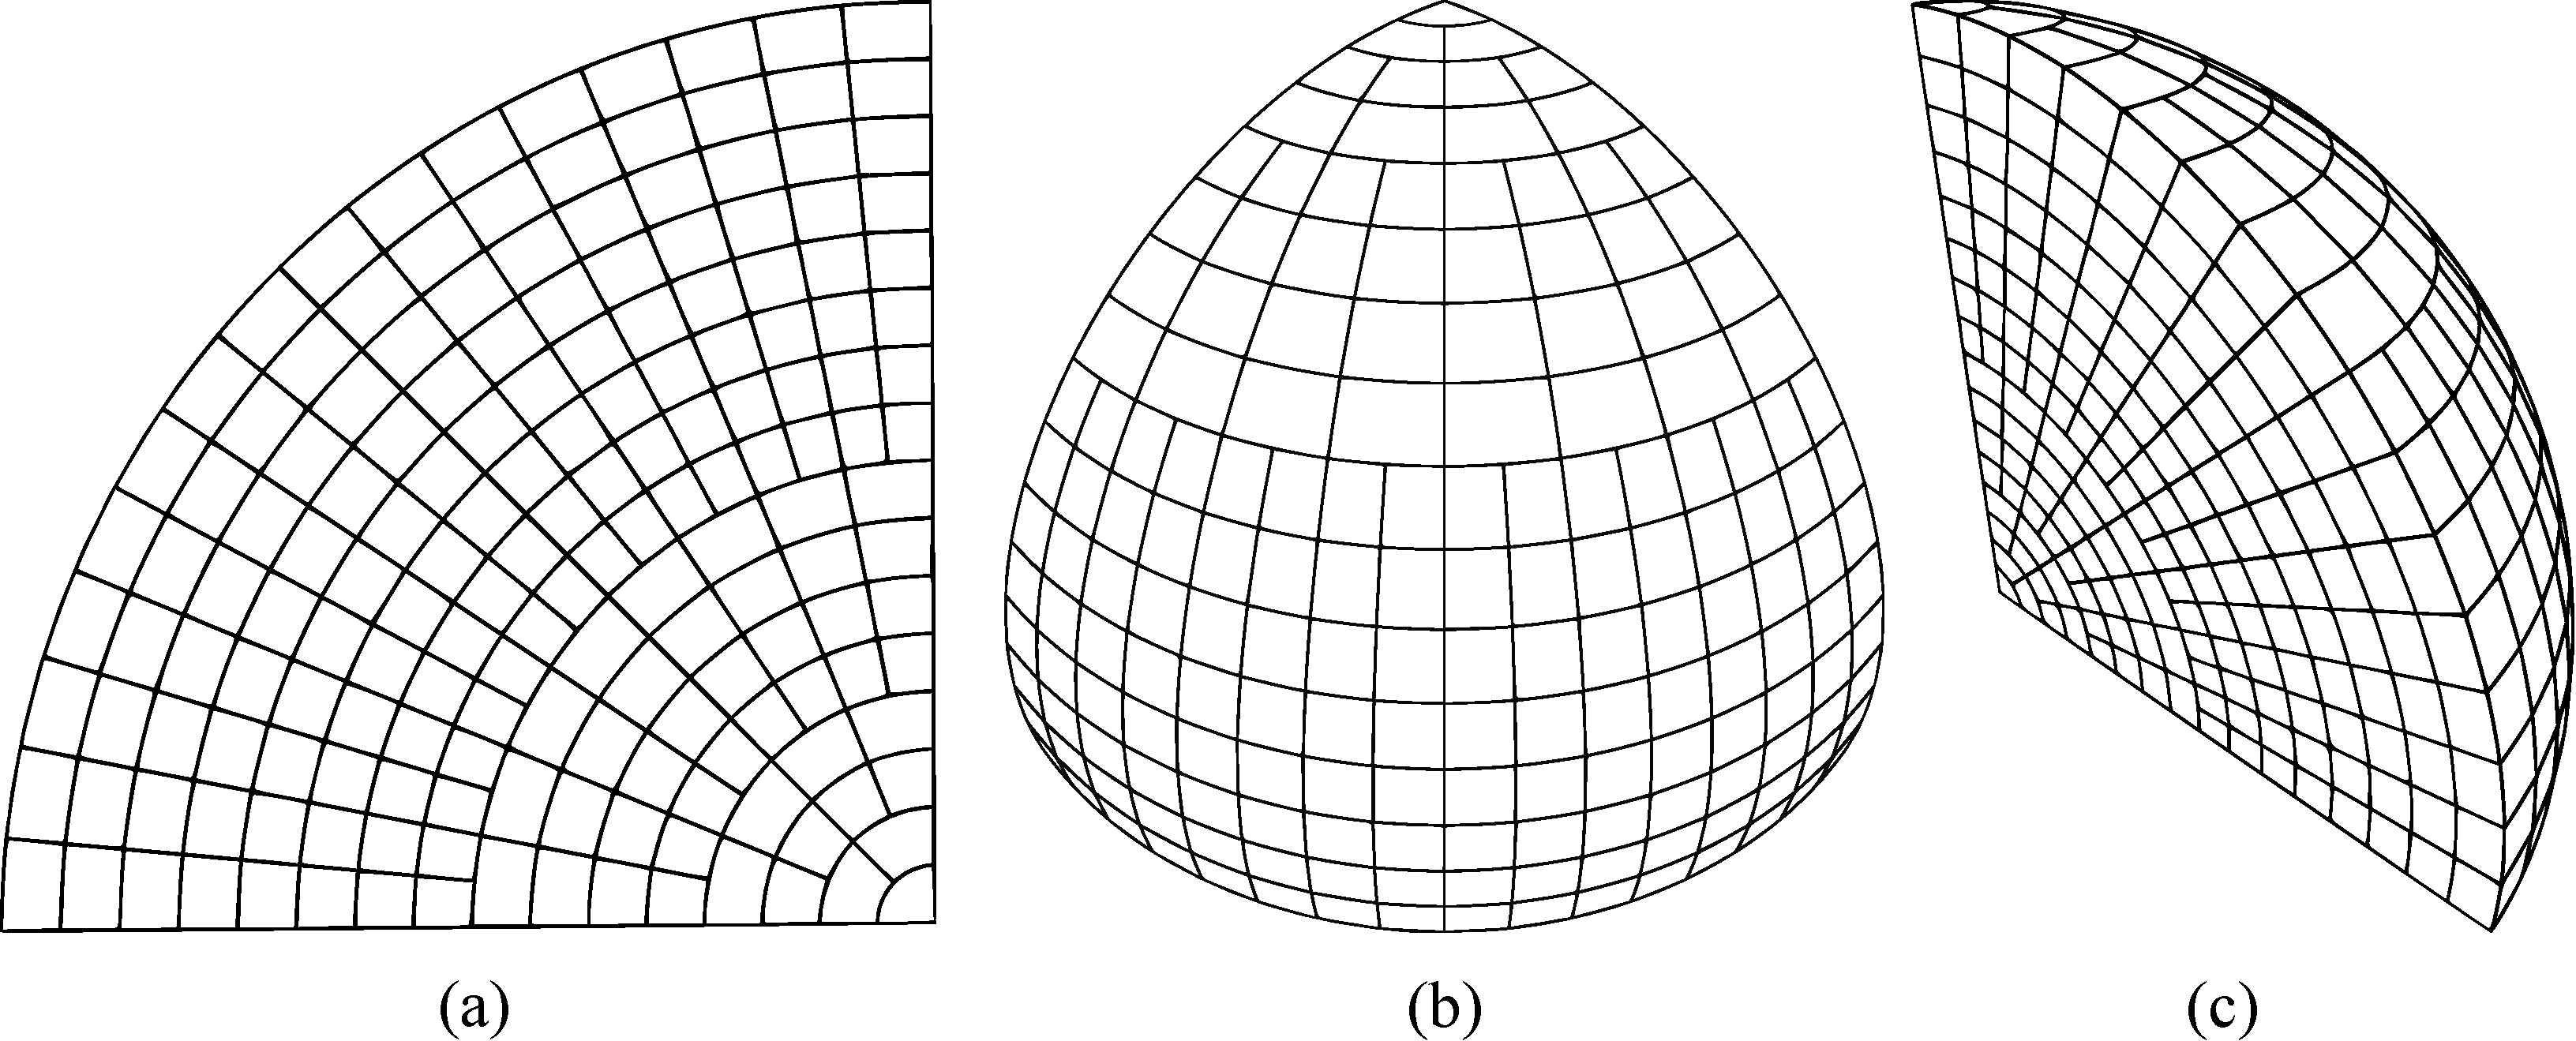
\includegraphics[width=\textwidth]{Fig2.pdf}
	\caption{One octant of an SDOG grid after four levels of subdivision viewed (a) from the side, (b) from the front, and (c) at an angle.
		Compared to a 3D LLG, cells are much more uniform in size and have much better compactness.
		Refer to Section~\ref{sec:results} for a detailed analysis of the volume preserving and compactness properties of SDOG}
	\label{fig:sdog}
\end{figure}


We first provide a brief explanation of SDOG construction and refinement as presented in~\cite{yu2009sdog}.
SDOG is an extension of the traditional octree to a spherical, as opposed to Euclidean, volume.
A sphere with twice the radius of the Earth is initially divided into eight equal octants via the equatorial plane and two perpendicular meridian planes.
These octants are taken to be the coarsest cells of the grid and are then subdivided to create more fine discretizations of the sphere.
An SDOG octant after four subdivisions can be seen in Figure~\ref{fig:sdog}.


\begin{figure}[tbp]
	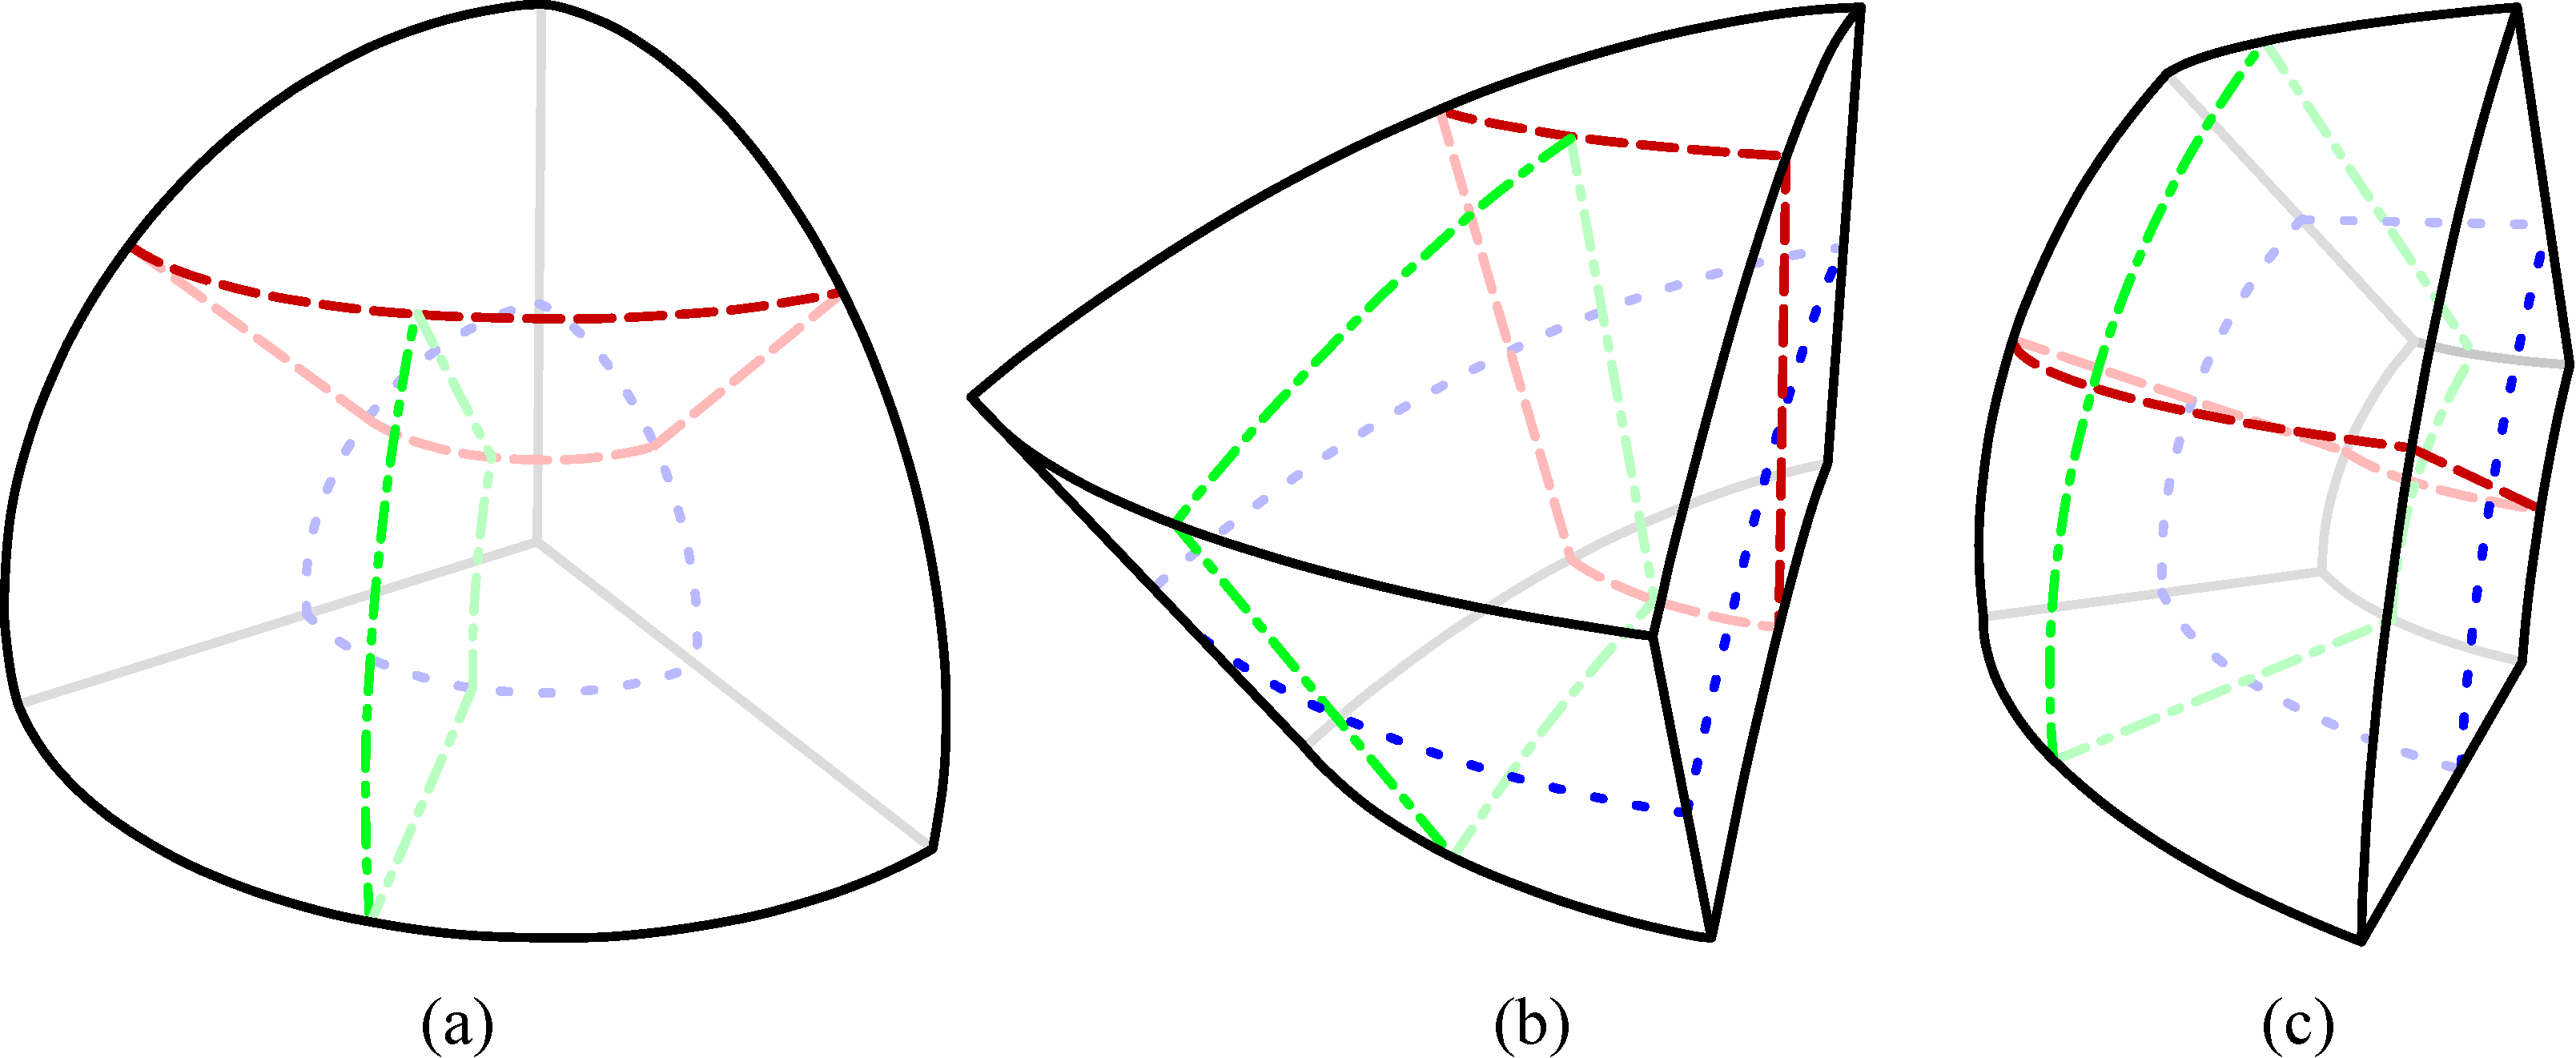
\includegraphics[width=\textwidth]{Fig3.pdf}
	\caption{Location and extent of splitting surfaces in SDOG subdivision for (a) SG cells, (b) LG cells, and (c) NG cells.
		Only NG cells have all three splitting surfaces fully subdivide the cell into eight children, and make up the majority of cells as the grid becomes more refined.}
	\label{fig:subRules}
\end{figure}


SDOG cells (including octants) are subdivided using the midpoint of each spherical coordinate: latitude, longitude, and radius.
These midpoints create splitting surfaces that can be used to split parent cells into smaller children cells.
To prevent the degeneration in cell compactness and size near the poles and centre of the sphere seen in 3D LLGs (Figure~\ref{fig:3dllg}), the extent of these splitting surfaces and the number of resulting children cells depends on the shape, or class, of cell that is being divided.
The splitting surfaces for each type of SDOG cell are shown in Figure~\ref{fig:subRules}.
We call a splitting surface symmetric if it creates the same number and type(s) of cells on both sides; otherwise we call it degenerate.


Cells that extend to the centre of the sphere and to one of the poles are referred to as Sphere-degenerated Grid (SG) cells (Figure~\ref{fig:subRules}a) and include the original eight octants.
For these cells, the longitudinal splitting surface does not extend beyond the latitudinal one in the direction towards the pole.
Additionally, neither the latitudinal nor longitudinal splitting surfaces extend beyond the radial one in the direction towards the centre of the sphere.
The result of this subdivision is four children cells: another SG cell, one Latitude-degenerated Grid (LG) cell, and two Normal Grid (NG) cells.
LG and NG cells are described below.
Only the longitudinal splitting surface for SG cells is symmetric.


LG cells (Figure~\ref{fig:subRules}b) are similar to SG ones, except that they only extend to one of the poles and not the centre of the sphere.
Therefore, the longitudinal splitting surface does not extend beyond the latitudinal one in the direction towards the pole.
This subdivision results in six children cells: two LG cells and four NG cells.
The longitudinal and radial splitting surfaces for LG cells are symmetric.


NG cells (Figure~\ref{fig:subRules}c) extend to neither the pole nor the centre of the sphere and make up the majority of SDOG cells.
These cells are fully subdivided into eight children NG cells and are the regular case for SDOG subdivision.
All splitting surfaces for NG cells are symmetric.


\subsection{SDOG Indexing} \label{sec:sdog-indexing}
In order to identify and distinguish the cells of a grid, there needs to be a method to assign a unique index to each cell.
A good indexing scheme will allow for efficient data insertion, retrieval, and manipulation via a set of queries.
Examples of some of these queries are: point to cell, which give the index of the cell containing a given point; index inversion, which calculates a cell's location and geometry from the index; neighbourhood queries; and in the case of a hierarchical grid, hierarchy traversal to find parent and children cells.


Due to the fact that SDOG subdivision is based on the midpoints of spherical coordinates, an indexing scheme that is efficient for many of the above operations can be easily developed.
At any subdivision level, $k$, each cell can be given an integer index in each spherical coordinate ranging from zero to $2^{k} - 1$.
To address the degenerate subdivision of certain cells, these integer indices are modified appropriately with divisions by powers of two, which can be done quickly with bit shift operations.
The integer indices can then be linearized by various methods, one good choice being a Z-order curve \cite{morton1966computer} as used in \cite{yu2009sdog}.
A more detailed description of degenerate Z-order indexing for SDOG grids, including algorithms for point to cell and index inversion operations, can be found in \cite{yu2009coding}.


\subsection{Number of SDOG Cells} \label{sec:sdog-numCells}
Being able to analyze the number of cells in the grid at each level of subdivision is useful not only for measuring volume preserving properties---such as quickly calculating the average cell volume---but also for analyzing the behavior of the grid as the level of subdivision increases.
This type of analysis will prove useful in informing decisions about how to modify subdivision to improve volume preservation.


Due to the degenerate nature of SDOG subdivision, calculating the number of cells in the grid is more complicated than a simple exponential formulation.
Despite this, we can use the above subdivision rules to derive recursive definitions for the number of cells in an SDOG grid (or a single octant) at a given level of subdivision.
Let $S(k)$, $L(k)$, $N(k)$, and $T(k)$ be the number of SG, LG, NG, and total cells of an SDOG octant at subdivision level $k$, respectively.
There is only ever one SG cell in an SDOG octant, so trivially
%
\begin{equation}
S(k) = 1.
\label{eq:sg-num}
\end{equation}
%
We know each LG cell produces two new LG cells, and that the SG cell produces one new LG cell.
From this we can say
\begin{equation*}
L(k) = 2L(k-1) + 1 \quad\text{and}\quad L(1) = 1.
\label{eq:lg-recursive}
\end{equation*}
%
Similarly, each NG cell produces eight new NG cells, each LG cell produces four, and the SG cell produces two.
Thus
\begin{equation*}
N(k) = 8N(k-1) + 4L(k-1) + 2 \quad\text{and}\quad N(1) = 2.
\label{eq:ng-recursive}
\end{equation*}
%
$L(k)$ is a linear non-homogeneous recurrence which can be solved with standard techniques \cite{bellman1963differential}.
Solving and substituting into $N(k)$ we get another linear non-homogeneous recurrence which can be solved similarly.
Finally, we get the closed forms:
%
\begin{equation}
L(k) = 2^{k} - 1,
\label{eq:lg-closed}
\end{equation}
%
\begin{equation}
N(k) = \frac{1}{21} \left( 7*2^{k} + 8^{k+1} + 6 \right) - 2^{k}, \quad\text{and}
\label{eq:ng-closed}
\end{equation}
%
\begin{equation}
T(k) = S(k) + L(k) + N(k) = \frac{1}{21} \left( 7*2^{k} + 8^{k+1} + 6 \right).
\label{eq:t-closed}
\end{equation}
%
As far as we are aware, these formulations have not been provided in any of the existing literature on SDOG.


\subsection{Geometry of SDOG Cells} \label{sec:sdog-geometry}
In order to measure the volume preservation properties of SDOG and its modifications, it is necessary to be able to measure the volume of individual cells in the grid.
Since each SDOG cell can be expressed as a range of each spherical coordinate (latitude $\phi$, longitude $\lambda$, and radius $r$), calculating the volume of an individual cell is a straightforward task.
Note that we use the geographic convention for spherical coordinates in this paper.
Let the subscripts $2$ and $1$ denote the maximum and minimum of a given spherical coordinate for an SDOG cell, then the volume is given by \cite{yu2009sdog}
%
\begin{equation}
V = \frac{1}{3} \left( \lambda_{2} - \lambda_{1} \right) \left(r_{2}^{3} - r_{1}^{3} \right) \left(\sin\phi_{2} - \sin\phi_{1} \right).
\label{eq:volume}
\end{equation}


In addition to the volume of a cell, surface area is another useful property to be able to measure.
Combined with the volume of cells, this allows us to measure the compactness of cells, which we use in Section \ref{sec:results} to help evaluate the consequences of our modifications.
From the fact that SDOG cells are subdivided using spherical coordinates, each face of a cell is a section of a simple geometric shape.
Faces created by radial splitting surfaces are spherical, with surface area given by
%
\begin{equation}
r^{2} \left( \lambda_{2} - \lambda_{1} \right) \left( \sin\phi_{2} - \sin\phi_{1} \right).
\end{equation}
%
Faces created by longitudinal splitting surfaces are the difference of two circular sectors, and have an area of
\begin{equation}
\frac{1}{2} \left( \phi_{2} - \phi_{1} \right) \left( r_{2}^{2} - r_{1}^{2} \right).
\end{equation}
%
Finally, faces created by latitudinal splitting surfaces lie on a cone, with a surface area of
\begin{equation}
\frac{1}{2} \cos\phi \left( \lambda_{2} - \lambda_{1} \right) \left( r_{2}^{2} - r_{1}^{2} \right).
\end{equation}


\section{Modified SDOG Subdivision} \label{sec:method}
%\subsection{Ideal Placement of Splitting Surfaces}
%\subsection{Blending Functions}

\begin{figure}[tbp]
	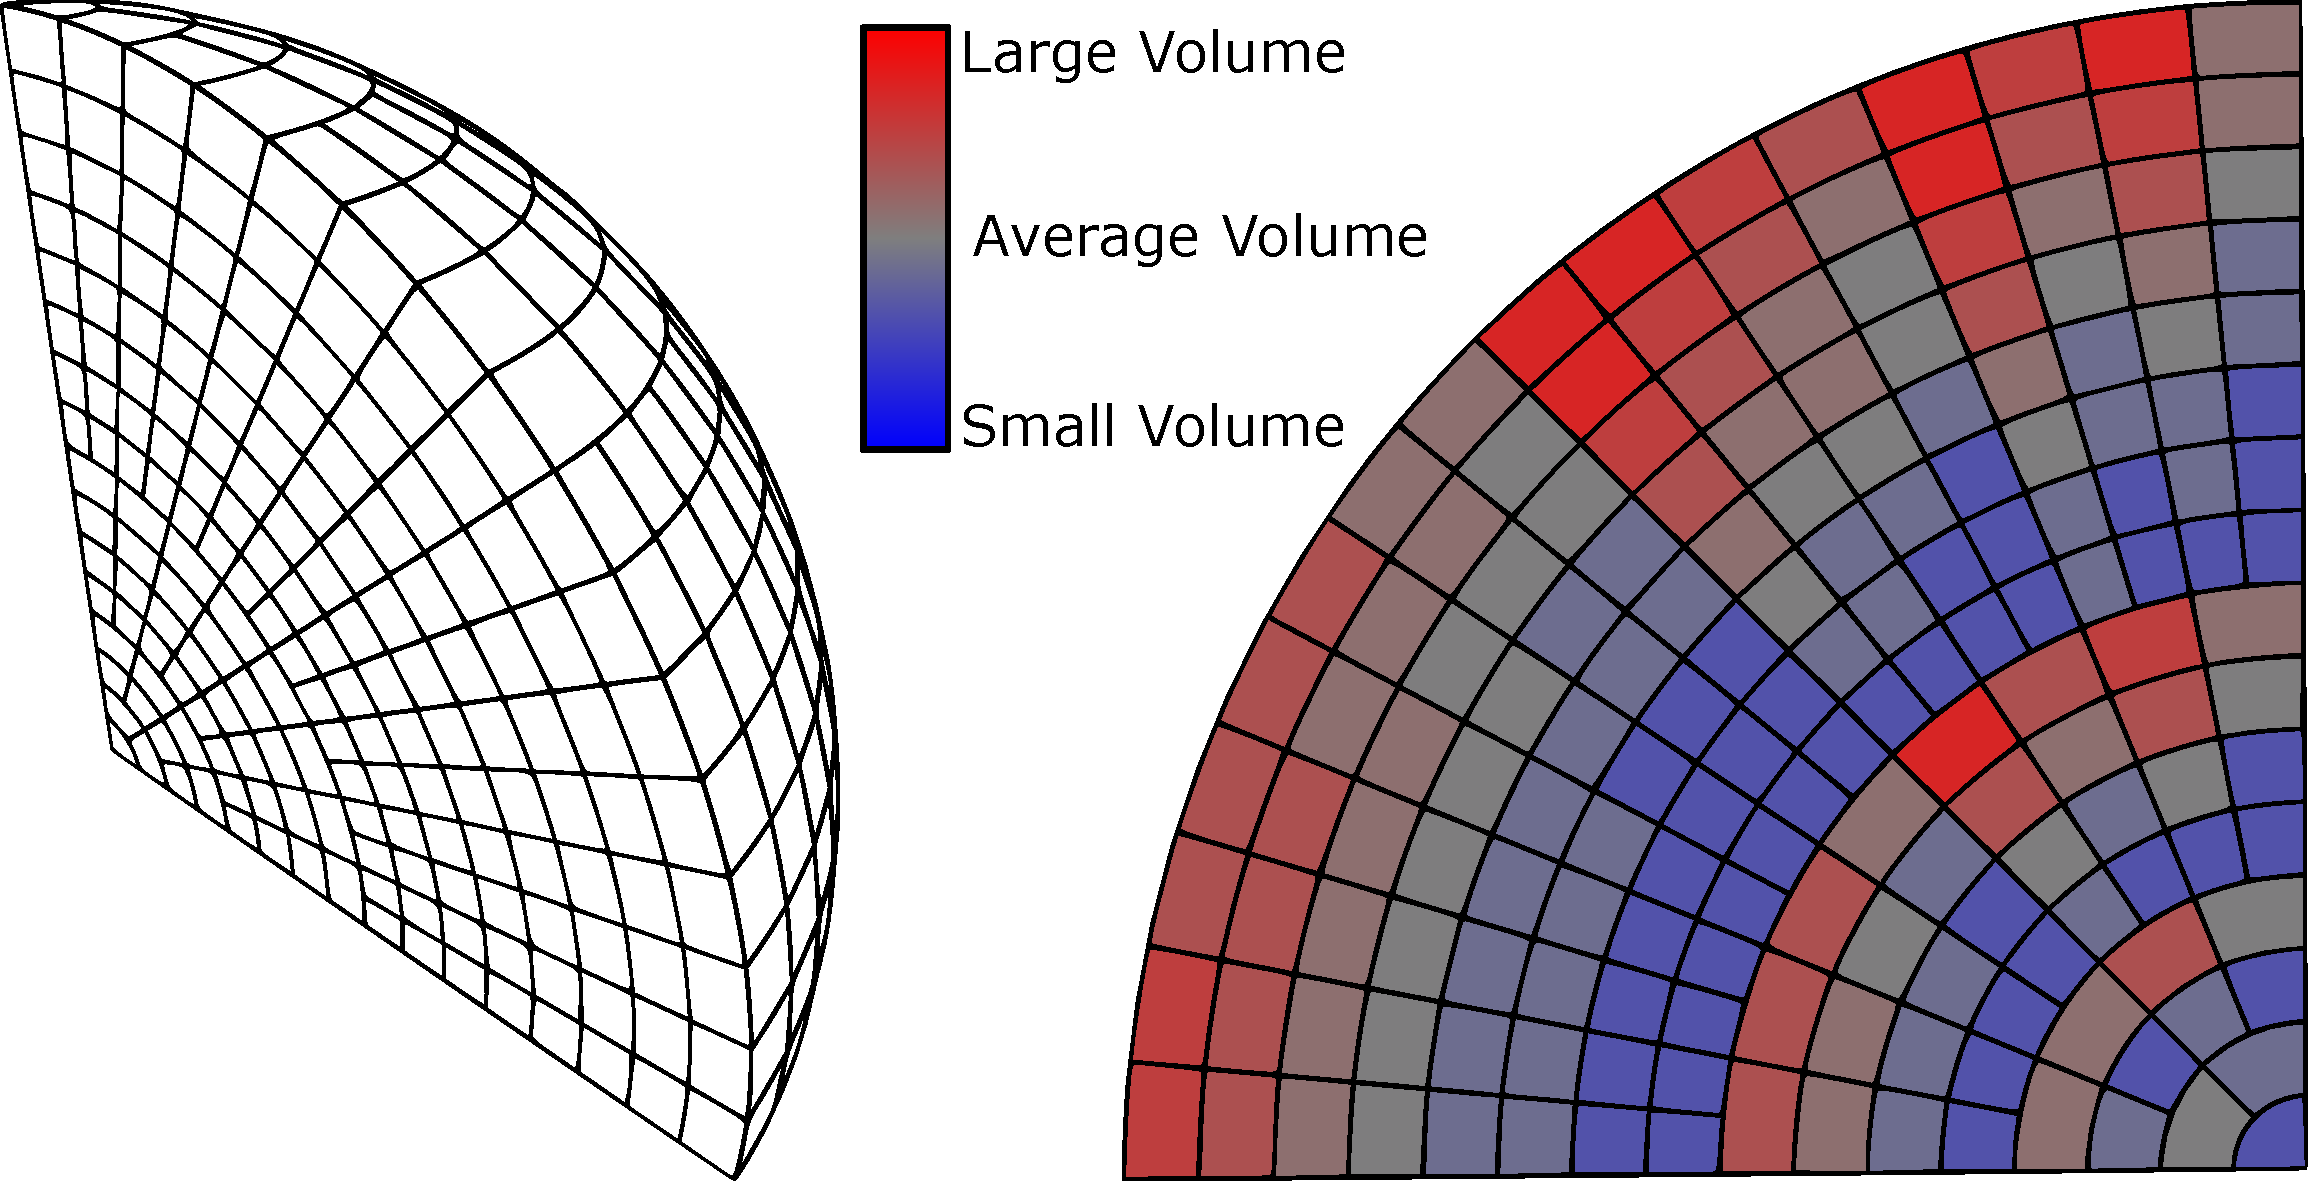
\includegraphics[width=0.85\textwidth]{Fig4.pdf}
	\caption{Distribution of cell volumes in an octant after four levels of conventional SDOG subdivision}
	\label{fig:sdog-vol}
\end{figure}


The main goal of this work is to modify SDOG in such a way as to improve volume preservation while minimizing the impact on other desired properties of the grid.
To aid in this task, we have developed a visualization framework for displaying and modifying SDOG grids.
This framework allows for changes to subdivision to be quickly implemented and allows visual analysis of said modifications.
All of the figures in the paper (except for the charts) were created using the output of this framework.
As an example and a baseline, the distribution of cell volumes in a conventional SDOG grid is visualized in Figure~\ref{fig:sdog-vol}.


As previously discussed, in conventional SDOG subdivision the location of the different splitting surfaces is always chosen to be at the midpoint of the respective spherical coordinate; we question if this should always be the case.
For an octree in Euclidean space this type of subdivision is desirable, as it generates children cells of identical size and shape.
In spherical space, however, this property does not transfer.
Using midpoints to subdivide cells makes for a simple subdivision scheme, but it makes no guarantees about the shape or size of the resulting children cells.


\begin{figure}[tbp]
	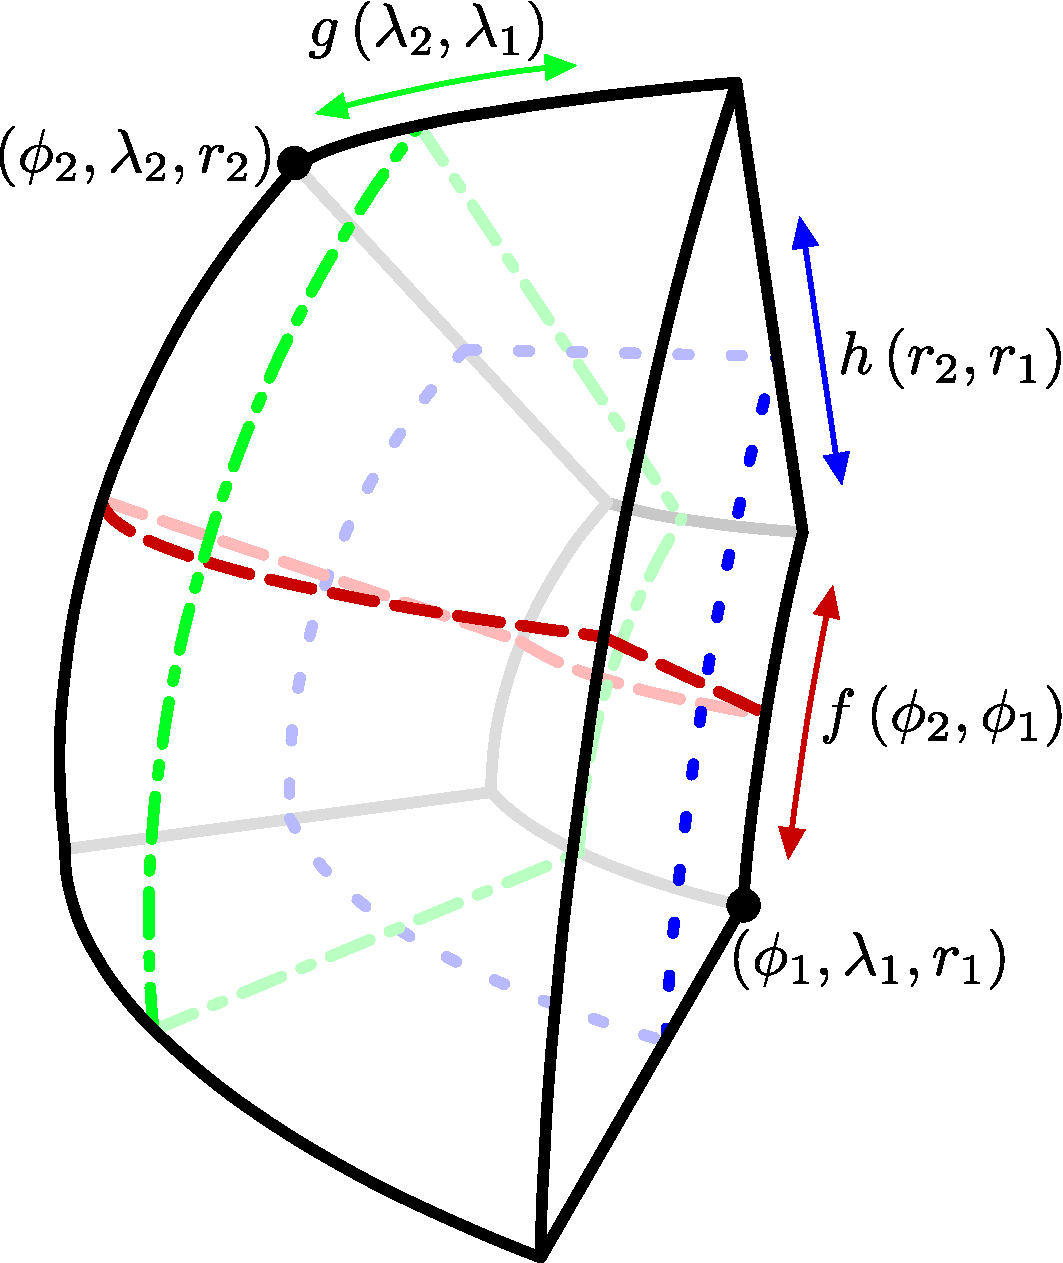
\includegraphics[width=0.5\textwidth]{Fig5.pdf}
	\caption{Each SDGO cell can be expressed as a range in each spherical coordinate, and the location of the splitting surface for each spherical coordinate can be expressed as a function of the maximum and minimum of the respective range.
		Here we show only an NG cell, however the same applies to SG and LG cells.
		The functions $f$, $g$, and $h$ serve as placeholders for any valid function that results in the output being strictly between the two inputs}
	\label{fig:functions}
\end{figure}


By allowing the location of the splitting surfaces to be adjusted, we can modify the shape and size of children cells and as a result affect the volume preservation, compactness, and other properties of the grid.
Let $c_{s}$ be the location of the splitting surface, where $c$ is one of $\left\lbrace \phi, \lambda, r \right\rbrace$, then one way to express the location of the splitting surfaces used for subdivision is as a convex combination of maximum and minimum values
%
\begin{equation} \label{eq:convex}
c_{s} = \alpha c_{2} + \left( 1-\alpha \right) c_{1}, \quad \alpha \in \left( 0, 1 \right),
\end{equation}
%
where we call $\alpha$ the splitting factor.
Conventional SDOG used midpoints (i.e.
$\alpha = \frac{1}{2}$) for each spherical coordinate when subdividing, regardless of cell type.
While a convex combination is the most straightforward, any function of the maximum and minimum such that the result is strictly between the two is a valid method for determining the location of the splitting surfaces (Figure~\ref{fig:functions}).
Thus, the location of splitting surfaces can be modified by changing this function, either by using a different value of $\alpha$, or by using a different function altogether.
Furthermore, the function used can be different for each cell type and spherical coordinate.


A useful function for improving volume preservation is one that results in one of the new ranges having a specific percentage of the volume of the original range.
We start with the radial splitting surface.
Referring to Eq.
(\ref{eq:volume}), let $p \in (0,1)$ be the percentage we wish for the lower range to have, then
%
\begin{equation*}
p \left( r_{2}^{3} - r_{1}^{3} \right) = r_{s}^{3} - r_{1}^{3}
\end{equation*}
%
\begin{equation*}
p r_{2}^{3} - p r_{1}^{3} = r_{s}^{3} - r_{1}^{3}
\end{equation*}
%
\begin{equation*}
r_{s}^{3} = p r_{2}^{3} + r_{1}^{3} - p r_{1}^{3}
\end{equation*}
%
\begin{equation*}
r_{s}^{3} = p r_{2}^{3} + \left( 1 - p \right) r_{1}^{3}
\end{equation*}
%
\begin{equation} \label{eq:radVol}
r_{s} = \sqrt[3]{ p r_{2}^{3} + \left( 1 - p \right) r_{1}^{3} }.
\end{equation}
%
The derivations for the latitudinal and longitudinal splitting surfaces follow the same, with results
%
\begin{equation} \label{eq:latVol}
\phi_{s} = \sin^{-1} \left( p \sin\phi_{2} + \left( 1 - p \right) \sin\phi_{1} \right), \quad\text{and}
\end{equation}
%
\begin{equation} \label{eq:longVol}
\lambda_{s} = p \lambda_{2} + \left( 1 - p \right) \lambda_{1}.
\end{equation}


The question then becomes which splitting surfaces can be modified, and in which ways, in order to improve the volume preservation of the grid.
We first look at which splitting surfaces should \textit{not} be modified.
From Eq.~(\ref{eq:longVol}) it is clear a longitudinal splitting surface at the midpoint will always split a cell exactly in half, and therefore since all longitudinal splitting surfaces are symmetric, they should not be changed.


\begin{figure}[tbp]
	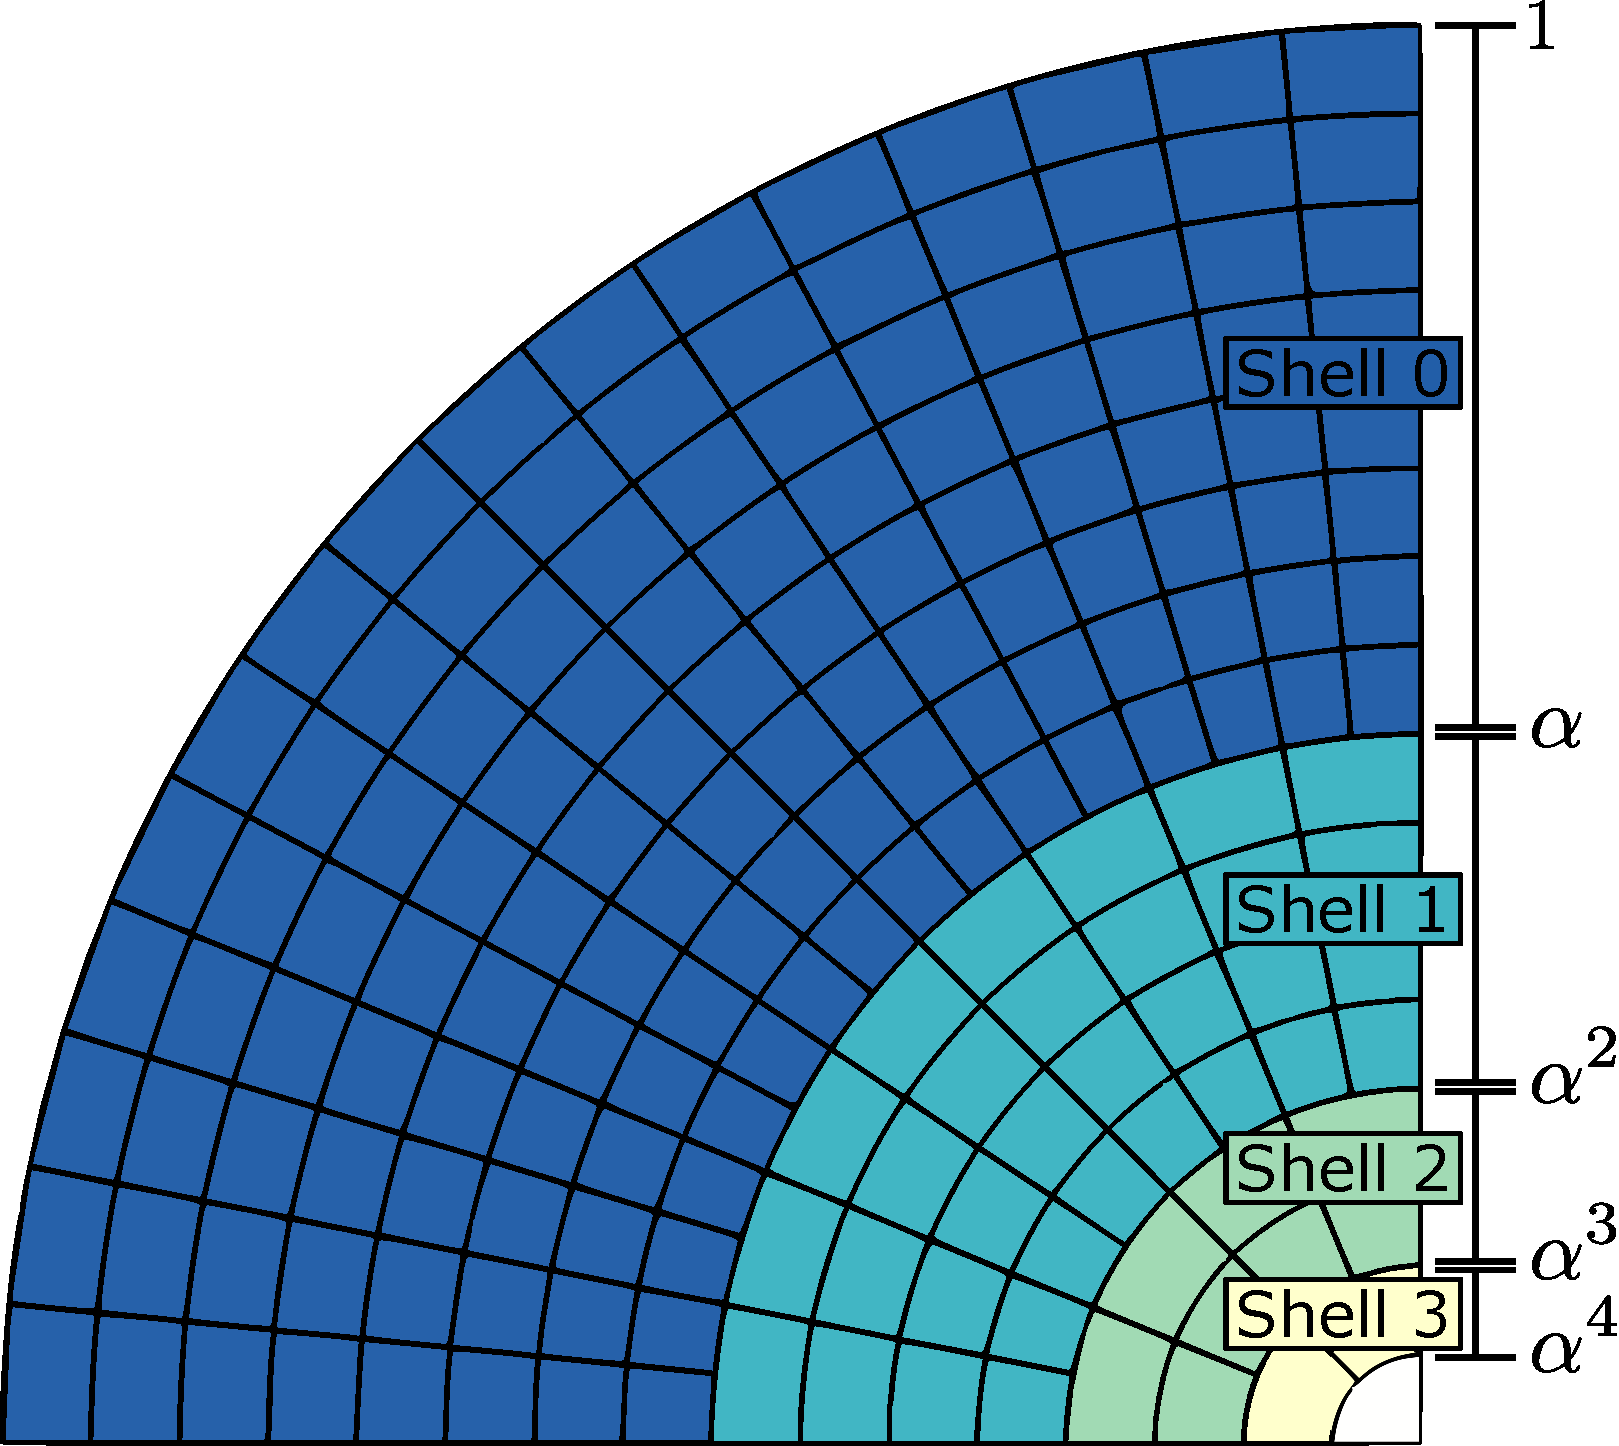
\includegraphics[width=0.6\textwidth]{Fig6.pdf}
	\caption{Spherical shells created by the radial splitting surfaces of SG cells.
		At $k$ levels of subdivision there are $k$ shells and one inner SG cell.
		These shells are similar and should have volume proportional to the number of cells they contain}
	\label{fig:sg-rad-splits}
\end{figure}


Less trivially, the radial splitting surface for SG cells should also be left at the midpoint.
Referring to Figure~\ref{fig:sg-rad-splits}, we can see that the radial splitting surfaces for SG cells separate the grid into spherical shells.
Shell $n$ has a volume proportional to
%
\begin{equation}
\alpha^{3n} - \alpha^{3 \left( n + 1 \right)},
\end{equation}
%
then the ratio of the volume between shell $n+1$ and $n$ is
%
\begin{equation}
\frac{ \alpha^{3 \left(n + 1 \right)} - \alpha^{3\left( n + 2 \right)} }{ \alpha^{3n} - \alpha^{3 \left( n + 1 \right)} } = \frac{ \alpha^{3} \alpha^{3n} \left( 1 - \alpha^{3} \right) }{ \alpha^{3n} \left( 1 - \alpha^{3} \right) } = \alpha^{3}.
\end{equation}
%
From the self similar nature of SDOG subdivision, we know that the cells in shell $n$ are simply the cells of shell $n+1$ subdivided once.
We also know that in the limit, an SDOG grid at one level higher of subdivision will have eight times as many cells as the previous resolution $\left( \lim_{k \to \infty} \frac{ T(k+1) }{ T(k) }  = 8 \right)$.
Therefore, in order for cells in the grid to be close to equal volume, it must be that shell $n+1$ has one eighth the volume of shell $n$ (since it will have one eighth the number of cells), which occurs exactly when $\alpha = \frac{1}{2}$.


This leaves five possible splitting surfaces that can be modified: the radial splitting surface for LG and NG cells, and the latitudinal splitting surface for SG, LG, and NG cells.
An important decision then is whether to use convex combinations to calculate the location of these surfaces (Eq.~(\ref{eq:convex})), or to use the functions parameterized by the ratio of volumes (Eq.~(\ref{eq:radVol}) and (\ref{eq:latVol})).
This is akin to a stationary subdivision scheme in comparison to a non-stationary one.
A stationary scheme will maintain the simplicity of subdivision, however, offers less overall ability to improve volume preservation.
Because of this, we provide both a stationary and non-stationary set of modifications.


\subsection{Stationary Subdivision} \label{sec:method-stationary}
By constraining splitting surfaces to be calculated via convex combinations, there are more restrictions on which splitting surfaces should be modified.
An interesting property of SDOG subdivision is that if a cell subdivides symmetrically in a given spherical dimension, all children of that cell also subdivide symmetrically in that dimension.
Thus, symmetric splitting surfaces result in non-degenerate binary (in the given dimension) subdivision at all further levels of subdivision, and it becomes clear that using any other value than the midpoint results in divergence as the level of subdivision gets large.
Therefore, all symmetric splitting surfaces should be left at the midpoint, which leaves only the latitudinal splitting surface for SG and LG cells to be modified.
We use $\alpha_{\phi}^{SG}$ and $\alpha_{\phi}^{LG}$ to refer to the splitting factors used for calculating the location of these surfaces.


\begin{figure}[tbp]
	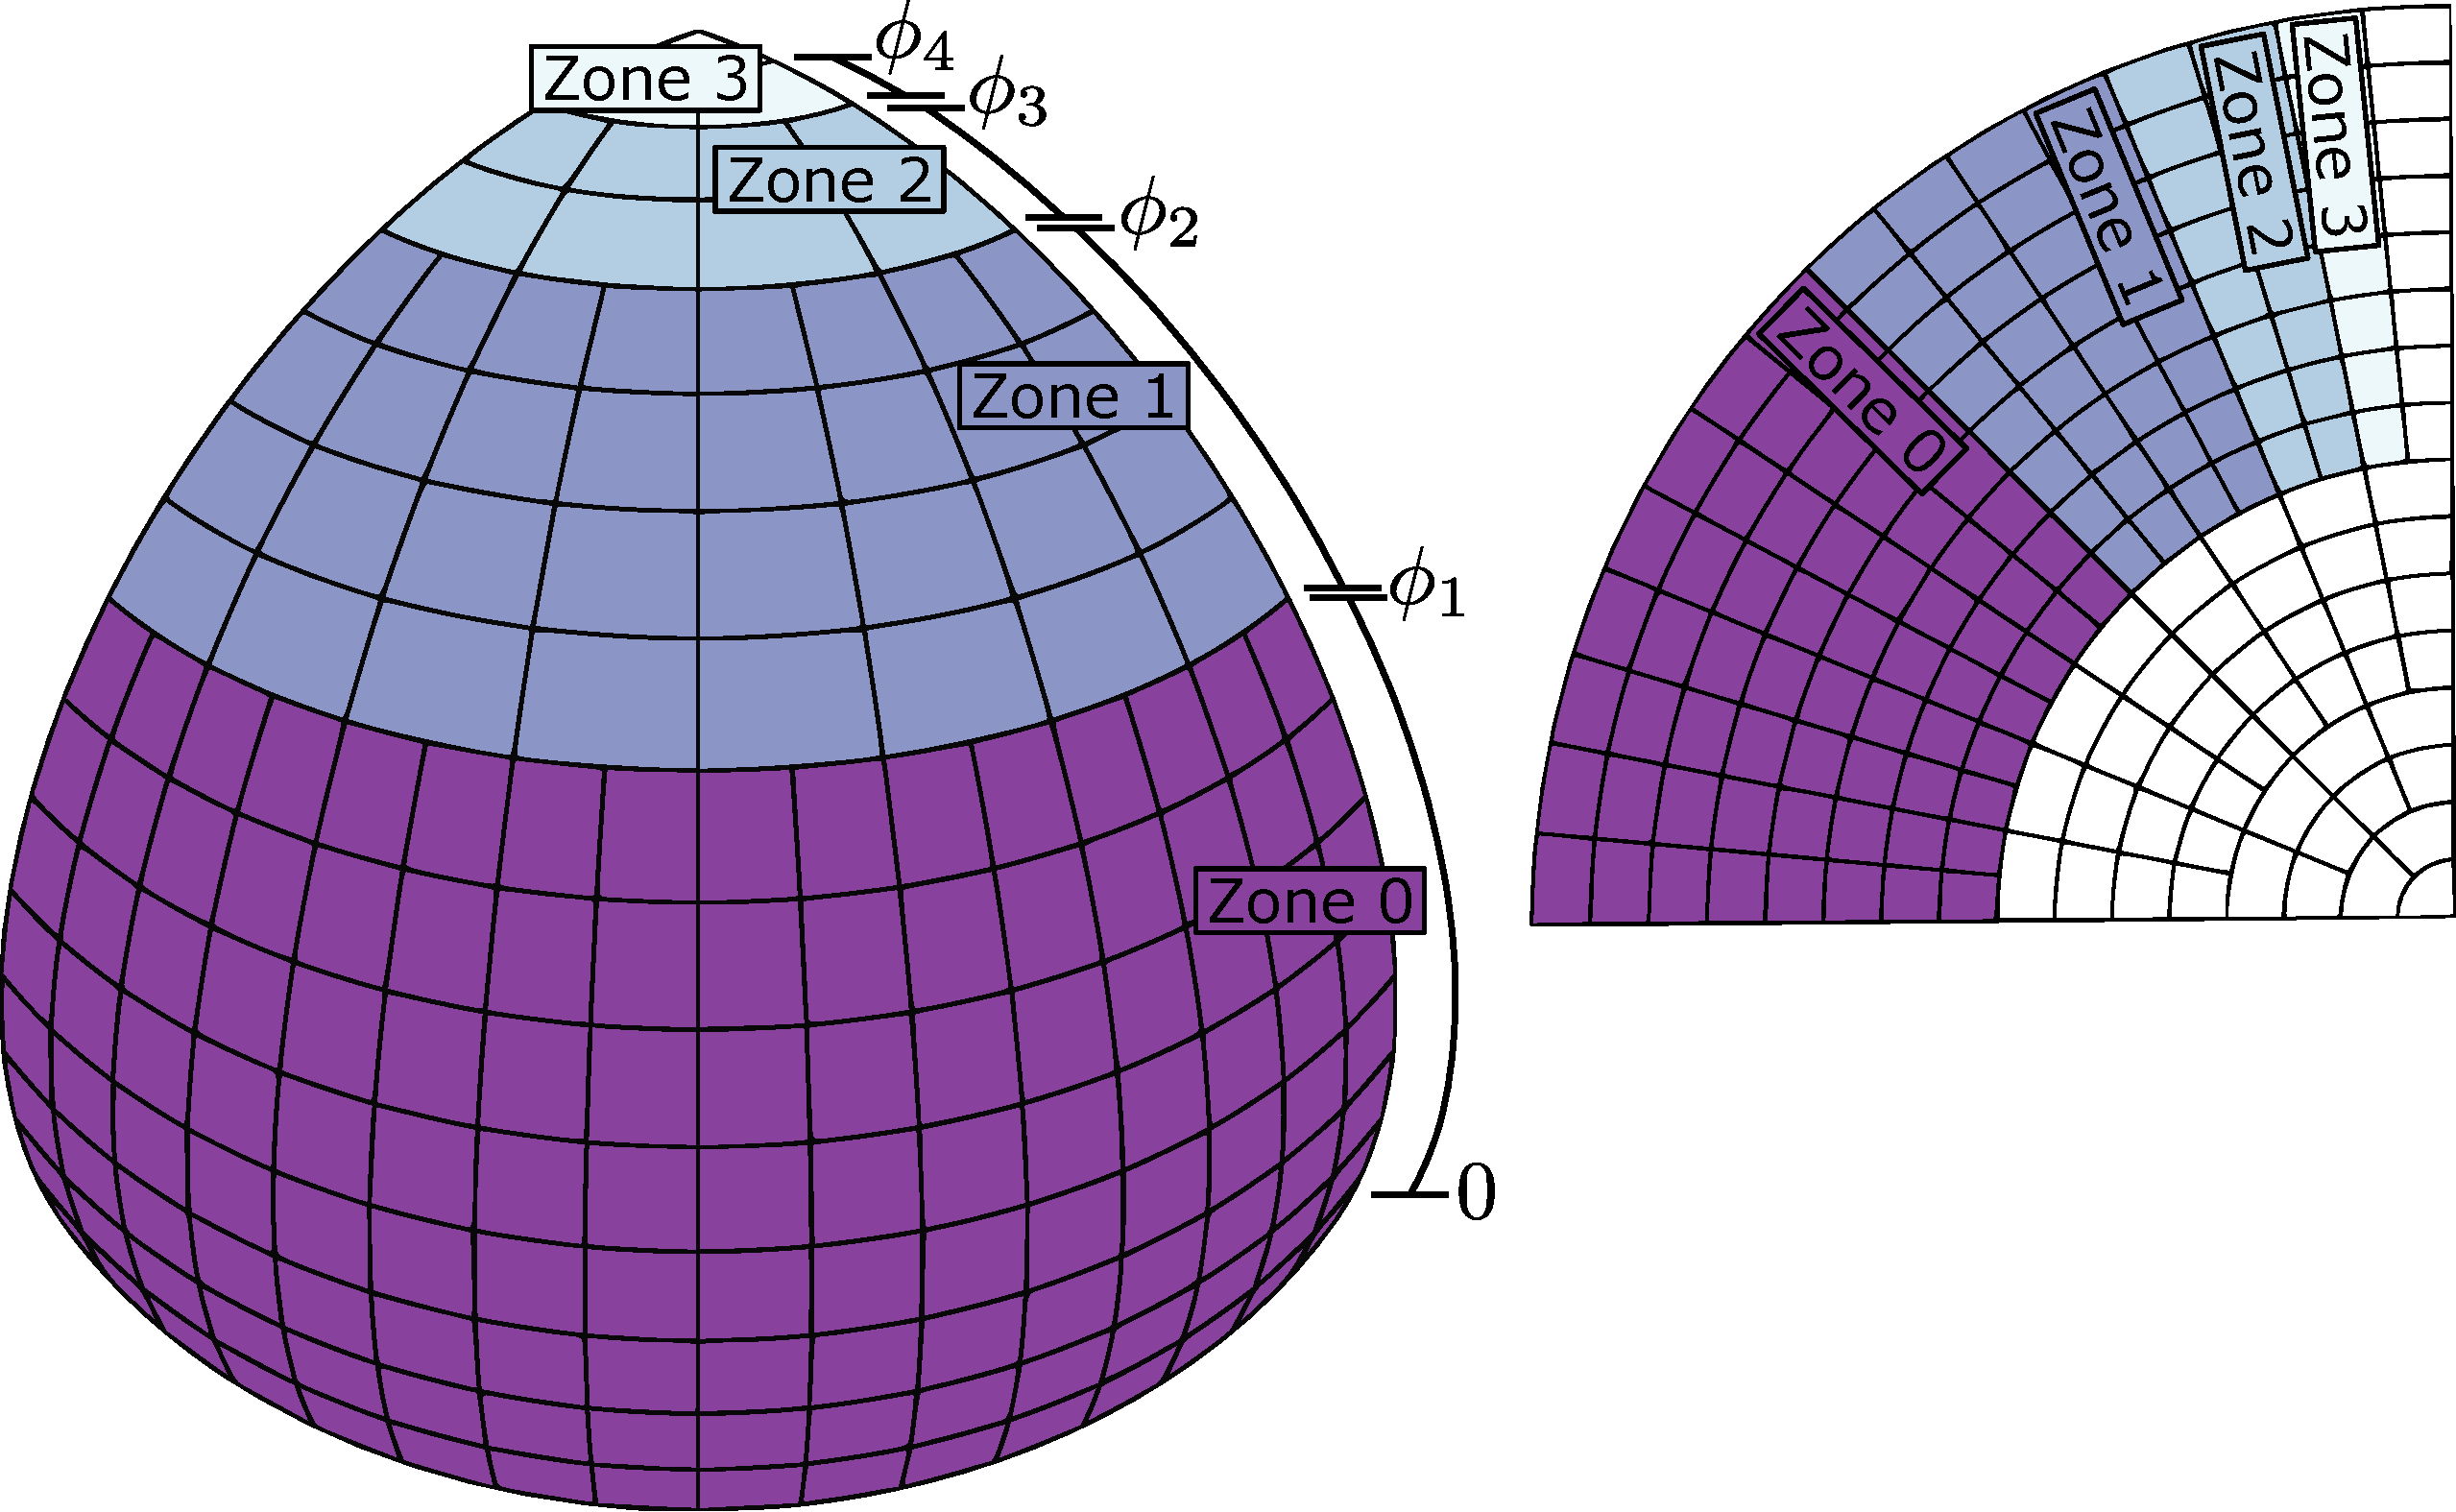
\includegraphics[width=0.9859\textwidth]{Fig7.pdf}
	\caption{Spherical zones created by the latitudinal splitting surfaces of SG and LG cells.
		At $k$ levels of subdivision there are $k$ zones and one upper stack of LG cells in the outer most shell.
		Each successively smaller shell has one fewer zones, until reaching the innermost SG cell.
		Zones in the same shell are not exactly similar, but are regular and should have volume proportional to the number of cells they contain}
	\label{fig:lat-splits}
\end{figure}


We first performed a simple search on the possible values of these splitting factors to see if it was possible to improve the volume preservation.
We found that volume preservation could be improved by certain values of $\alpha_{\phi}^{SG}$, however, it was always the case that $\alpha_{\phi}^{LG}$ was best left equal to one half.
To understand why this is the case, we look at where the ideal placements for these splitting surfaces would be if not constrained by convex combinations.
Notice that these two latitudinal splitting surfaces have a similar effect as the radial splitting surface for SG cells.
Referring now to Figure~\ref{fig:lat-splits}, we see that these splitting surfaces further divide the spherical shells into spherical zones.
Additionally, each zone is comprised entirely of NG cells.
From this fact we conclude that zone $n$ has exactly four times as many cells as zone $n+1$, and thus in the ideal case would have exactly four times the volume as well.
We can use Eq.~(\ref{eq:latVol}) to find these ideal locations using the proper value for $p$.
Zone $n$ has a percentage $\left( 1 - p \right)^{n} p$ of the initial volume of the octant, then setting the ratio between zone $n+1$ and $n$ to be equal to $\frac{1}{4}$ gives us $p = \frac{3}{4}$, and finally
%
\begin{equation} \label{eq:idealLat}
\phi_{s} = \sin^{-1} \left( \frac{3}{4} \sin\phi_{2} + \frac{1}{4} \sin\phi_{1} \right).
\end{equation}


From here, we can now see why the latitudinal splitting surfaces for LG cells should remain at the midpoint.
As $\phi_{1}$ approaches $\pm \frac{\pi}{2}$, this function is closely approximated by a convex combination with a factor of one half (see Appendix~\ref{app:lat}).
Thus, as the level of subdivision gets large, using $\alpha_{\phi}^{LG} = \frac{1}{2}$ approaches the ideal placement for the splitting surfaces, and thus is the ideal factor to use for a convex combination.


\begin{figure}[tbp]
	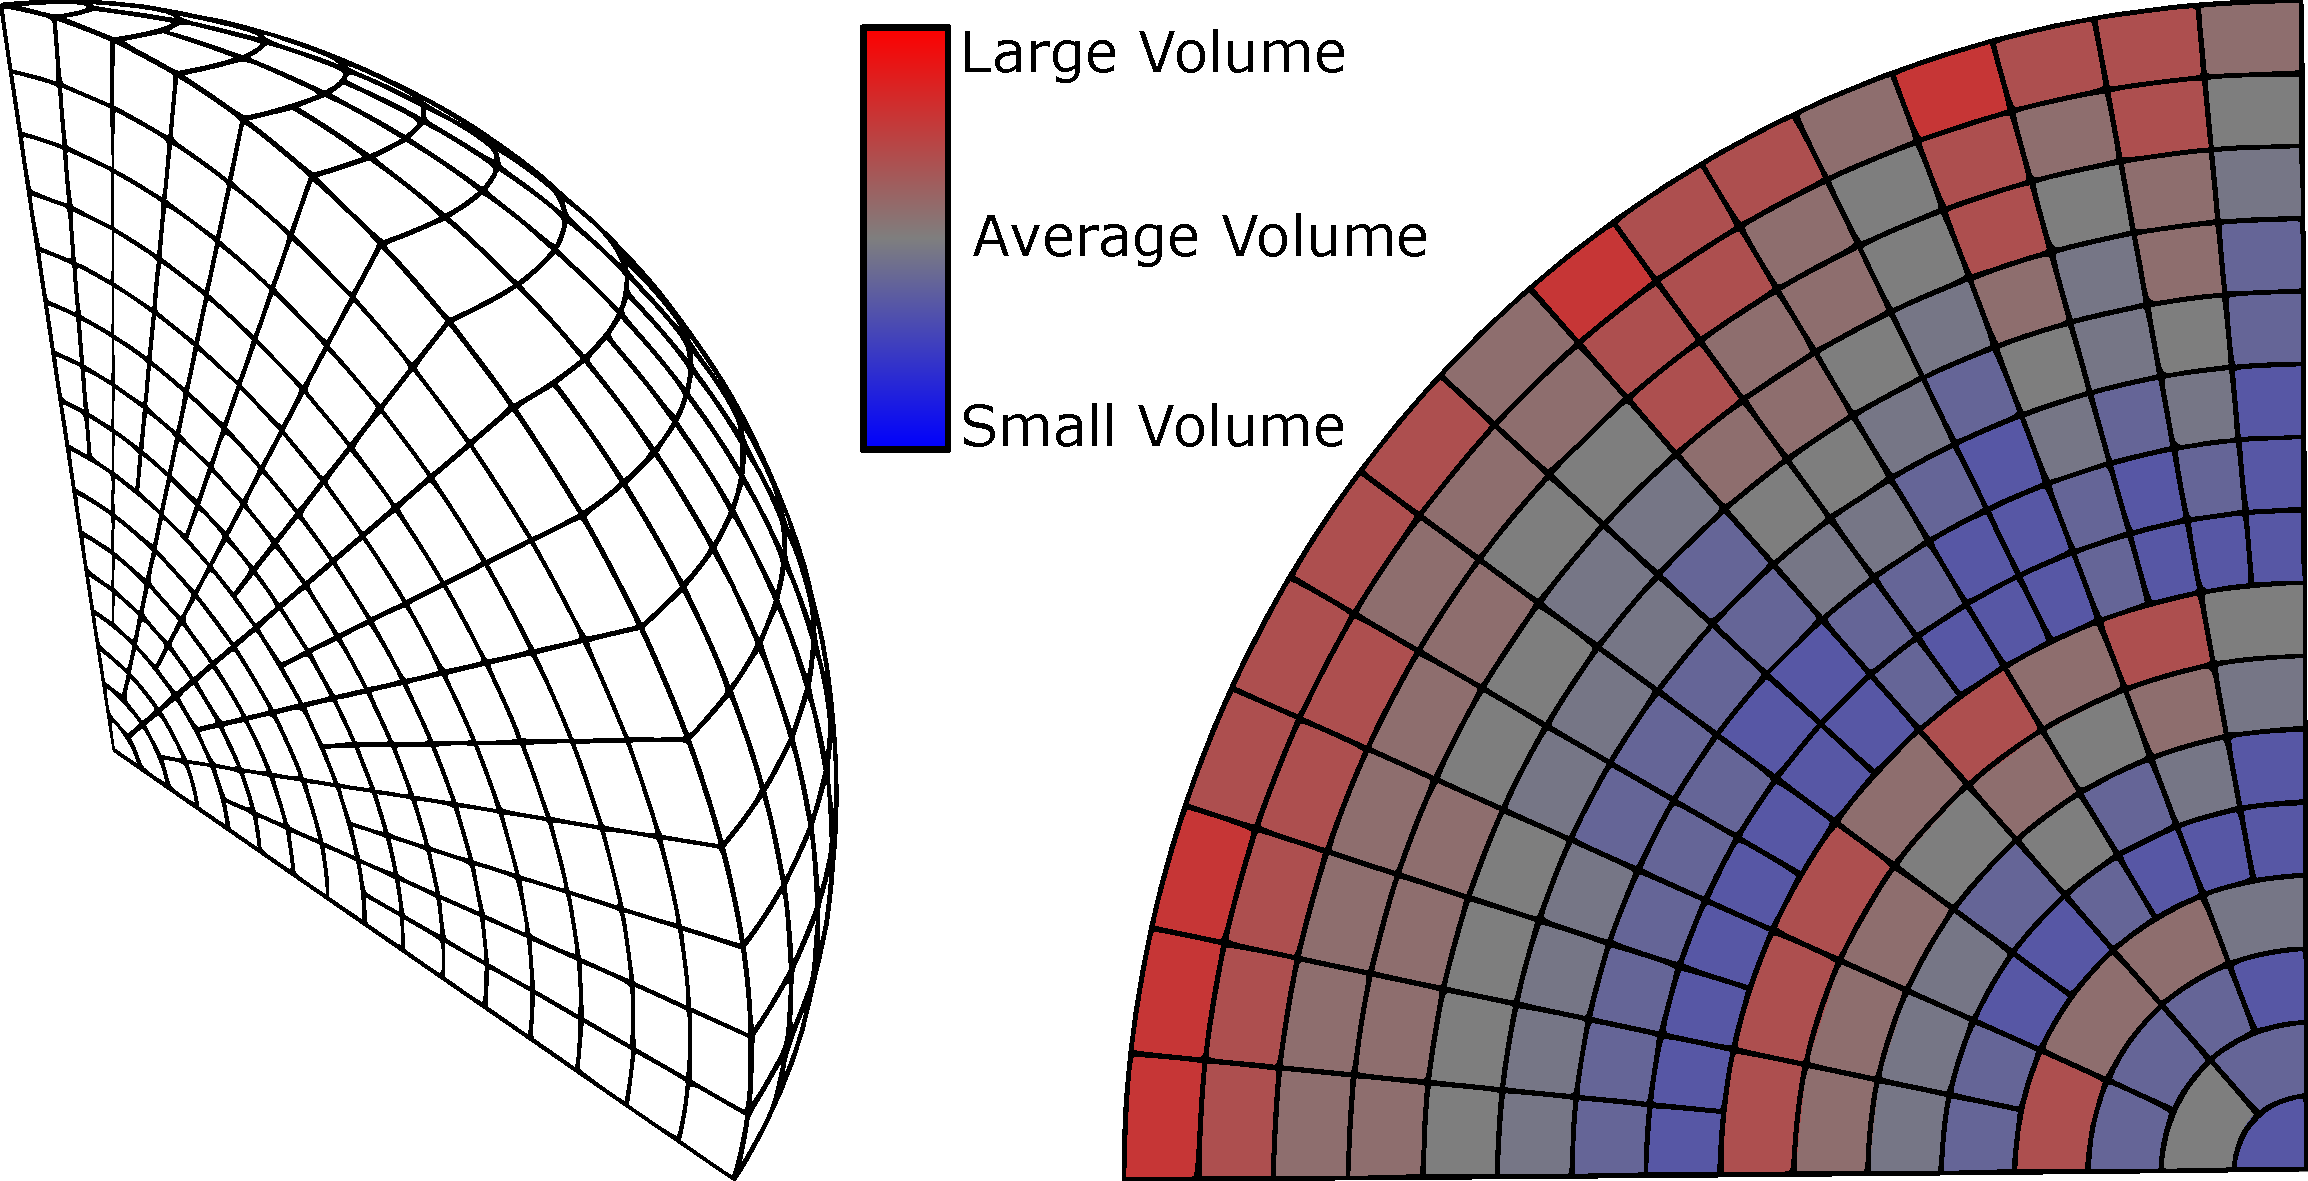
\includegraphics[width=0.85\textwidth]{Fig8.pdf}
	\caption{Results of the stationary scheme after four levels of subdivision using $\alpha_{\phi}^{SG} \approx 0.54$.
		Since only one type of splitting surface has been modified, the results are similar to that of conventional SDOG}
	\label{fig:stationary}
\end{figure}


We can also use this formulation to find the theoretical ideal placement for the latitudinal splitting surface of SG cells.
SG cells always have a minimum latitude of zero and a maximum of $\pm \frac{\pi}{2}$, thus Eq.~(\ref{eq:idealLat}) will always evaluate to plus or minus the same value.
Substituting back into Eq.~(\ref{eq:convex}) we get
%
\begin{equation} \label{eq:latValue}
\alpha_{\phi}^{SG} = \frac{ \sin^{-1} \left( \pm \frac{3}{4} \right) }{ \pm \frac{\pi}{2} } \approx 0.53989.
\end{equation}
%
The grid resulting from using this value can be seen in Figure~\ref{fig:stationary}.
Interestingly, our initial search also found $\alpha_{\phi}^{SG} = 0.57$ to perform well, even resulting in a slightly lower maximum difference in cell volumes than the theoretical ideal.
These findings are not necessarily in conflict, however, as the theoretical ideal results in much less variation in the volume of cells.
We compare these two schemes more closely in Section \ref{sec:results}.


\subsection{Non-Stationary Subdivision} \label{sec:method-nonStationary}
By not limiting splitting surfaces to be calculated using convex combinations, we are allowed much more control over subdivision and the resulting properties.
Using Eq~(\ref{eq:radVol}) and (\ref{eq:latVol}) to calculate the modifiable splitting surfaces, all that is needed is to determine the ideal value of $p$ for the different splitting surfaces and cell types.
We have already done this for the latitudinal splitting surfaces of SG and LG cells in Section \ref{sec:method-stationary} with Eq.~(\ref{eq:idealLat}).
Therefore, all that is left is the radial splitting surfaces for LG and NG cells, and the latitudinal one for NG cells.
However, since all of these remaining splitting surfaces are symmetric, we simply require that the volume on each side of these splitting surfaces be equal.
In other words, we can simply set $p = \frac{1}{2}$ for these remaining splitting surfaces.


\begin{figure}[tbp]
	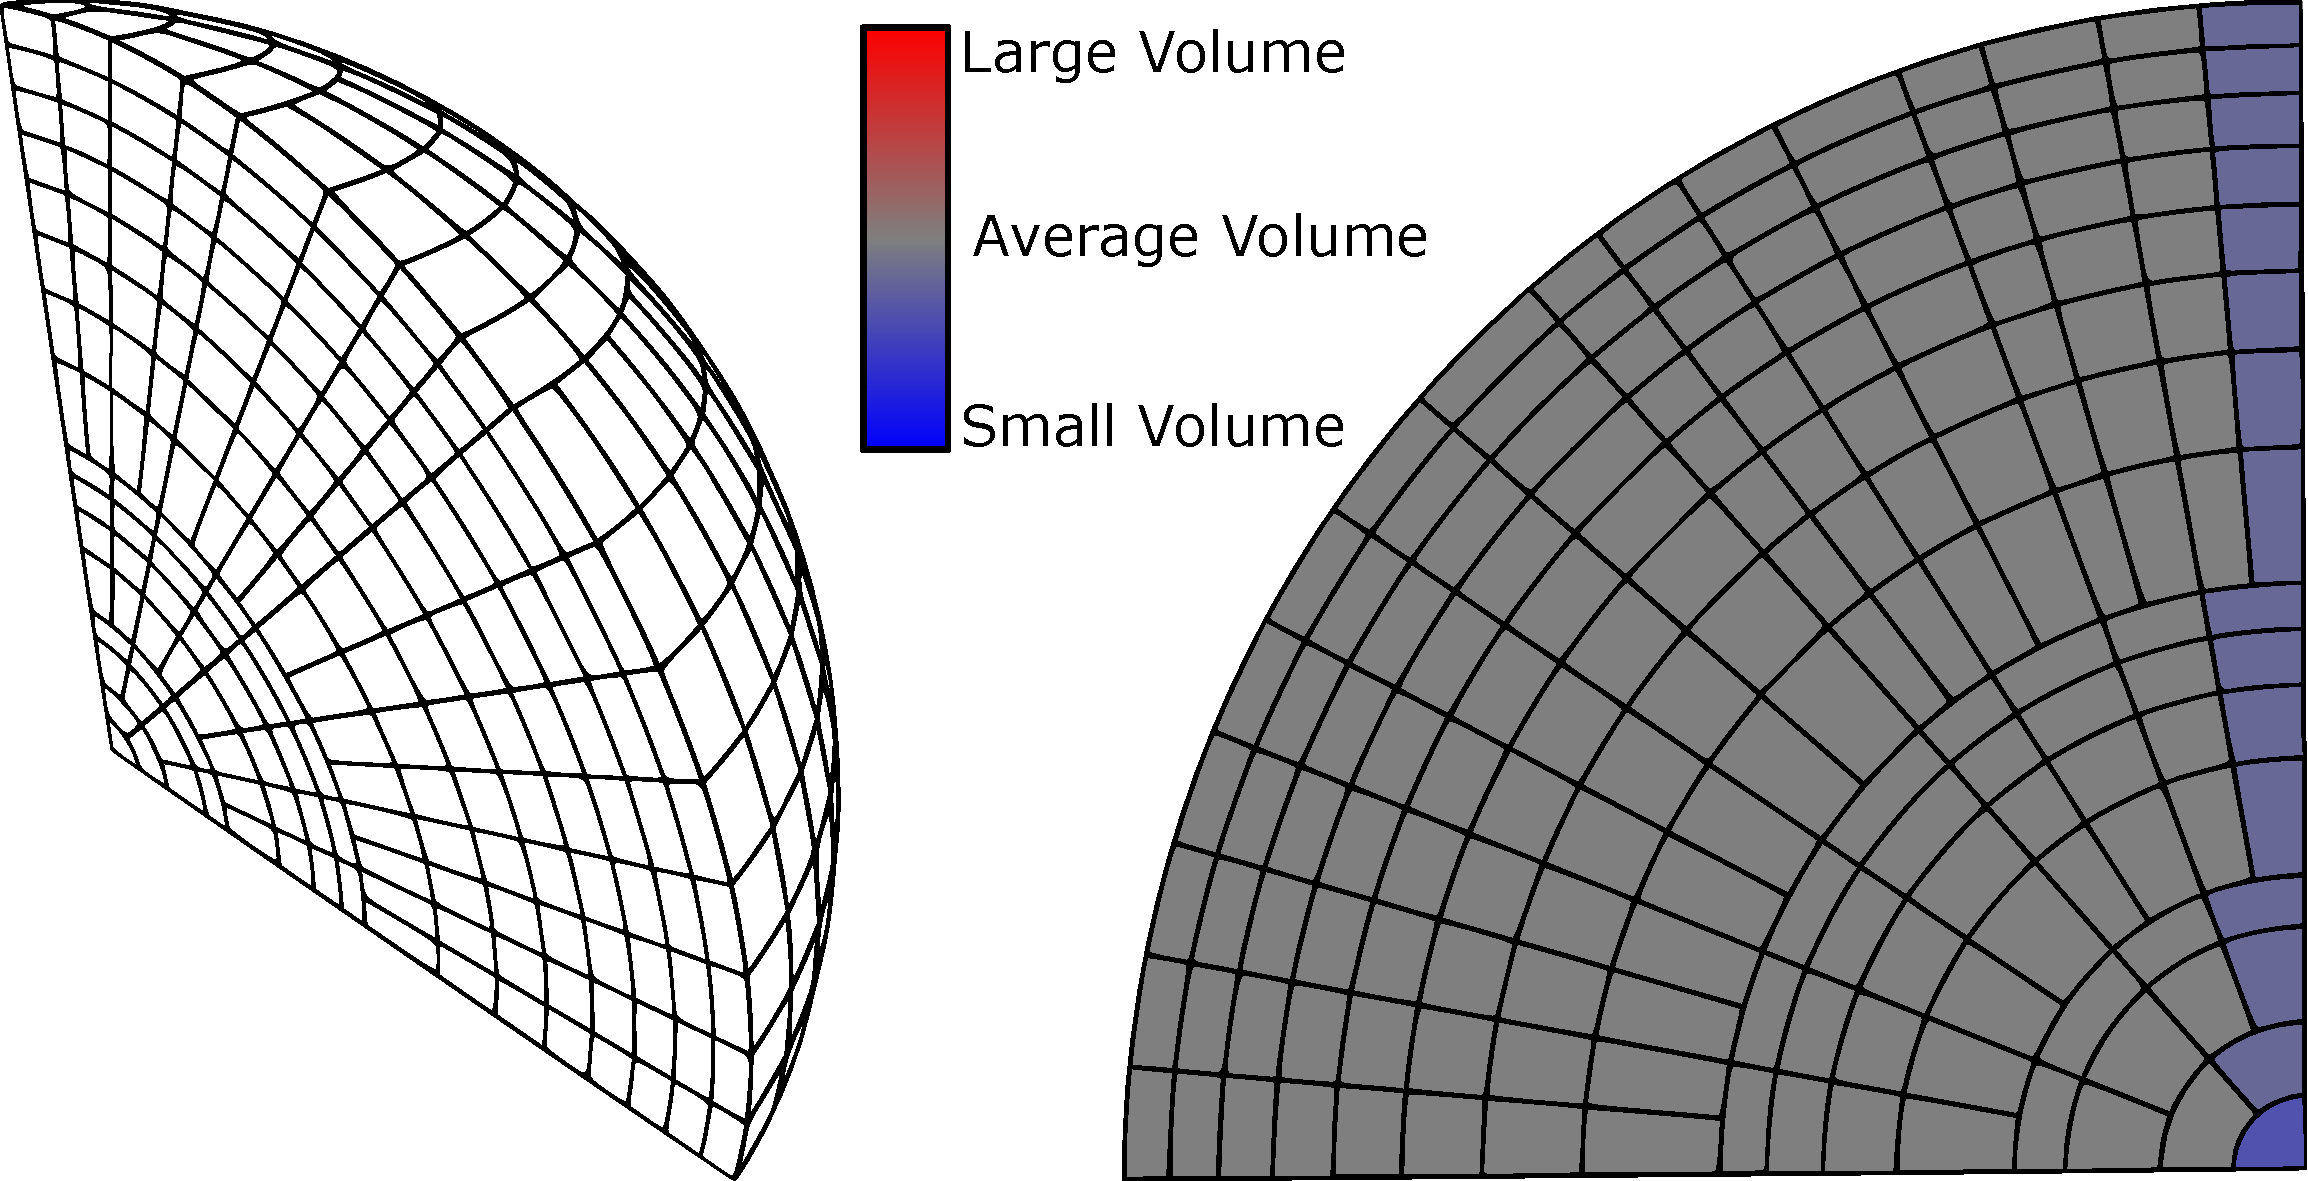
\includegraphics[width=0.85\textwidth]{Fig9.pdf}
	\caption{Results of the non-stationary scheme after four levels of subdivision using $\beta = 1$.
		All NG cells have exactly the same volume, with the LG and SG cells having a lower volume.
		Notice how the resulting NG cells are stretched and squashed in order to ensure they all have equal volume}
	\label{fig:perfect}
\end{figure}


\begin{figure}[tbp]
	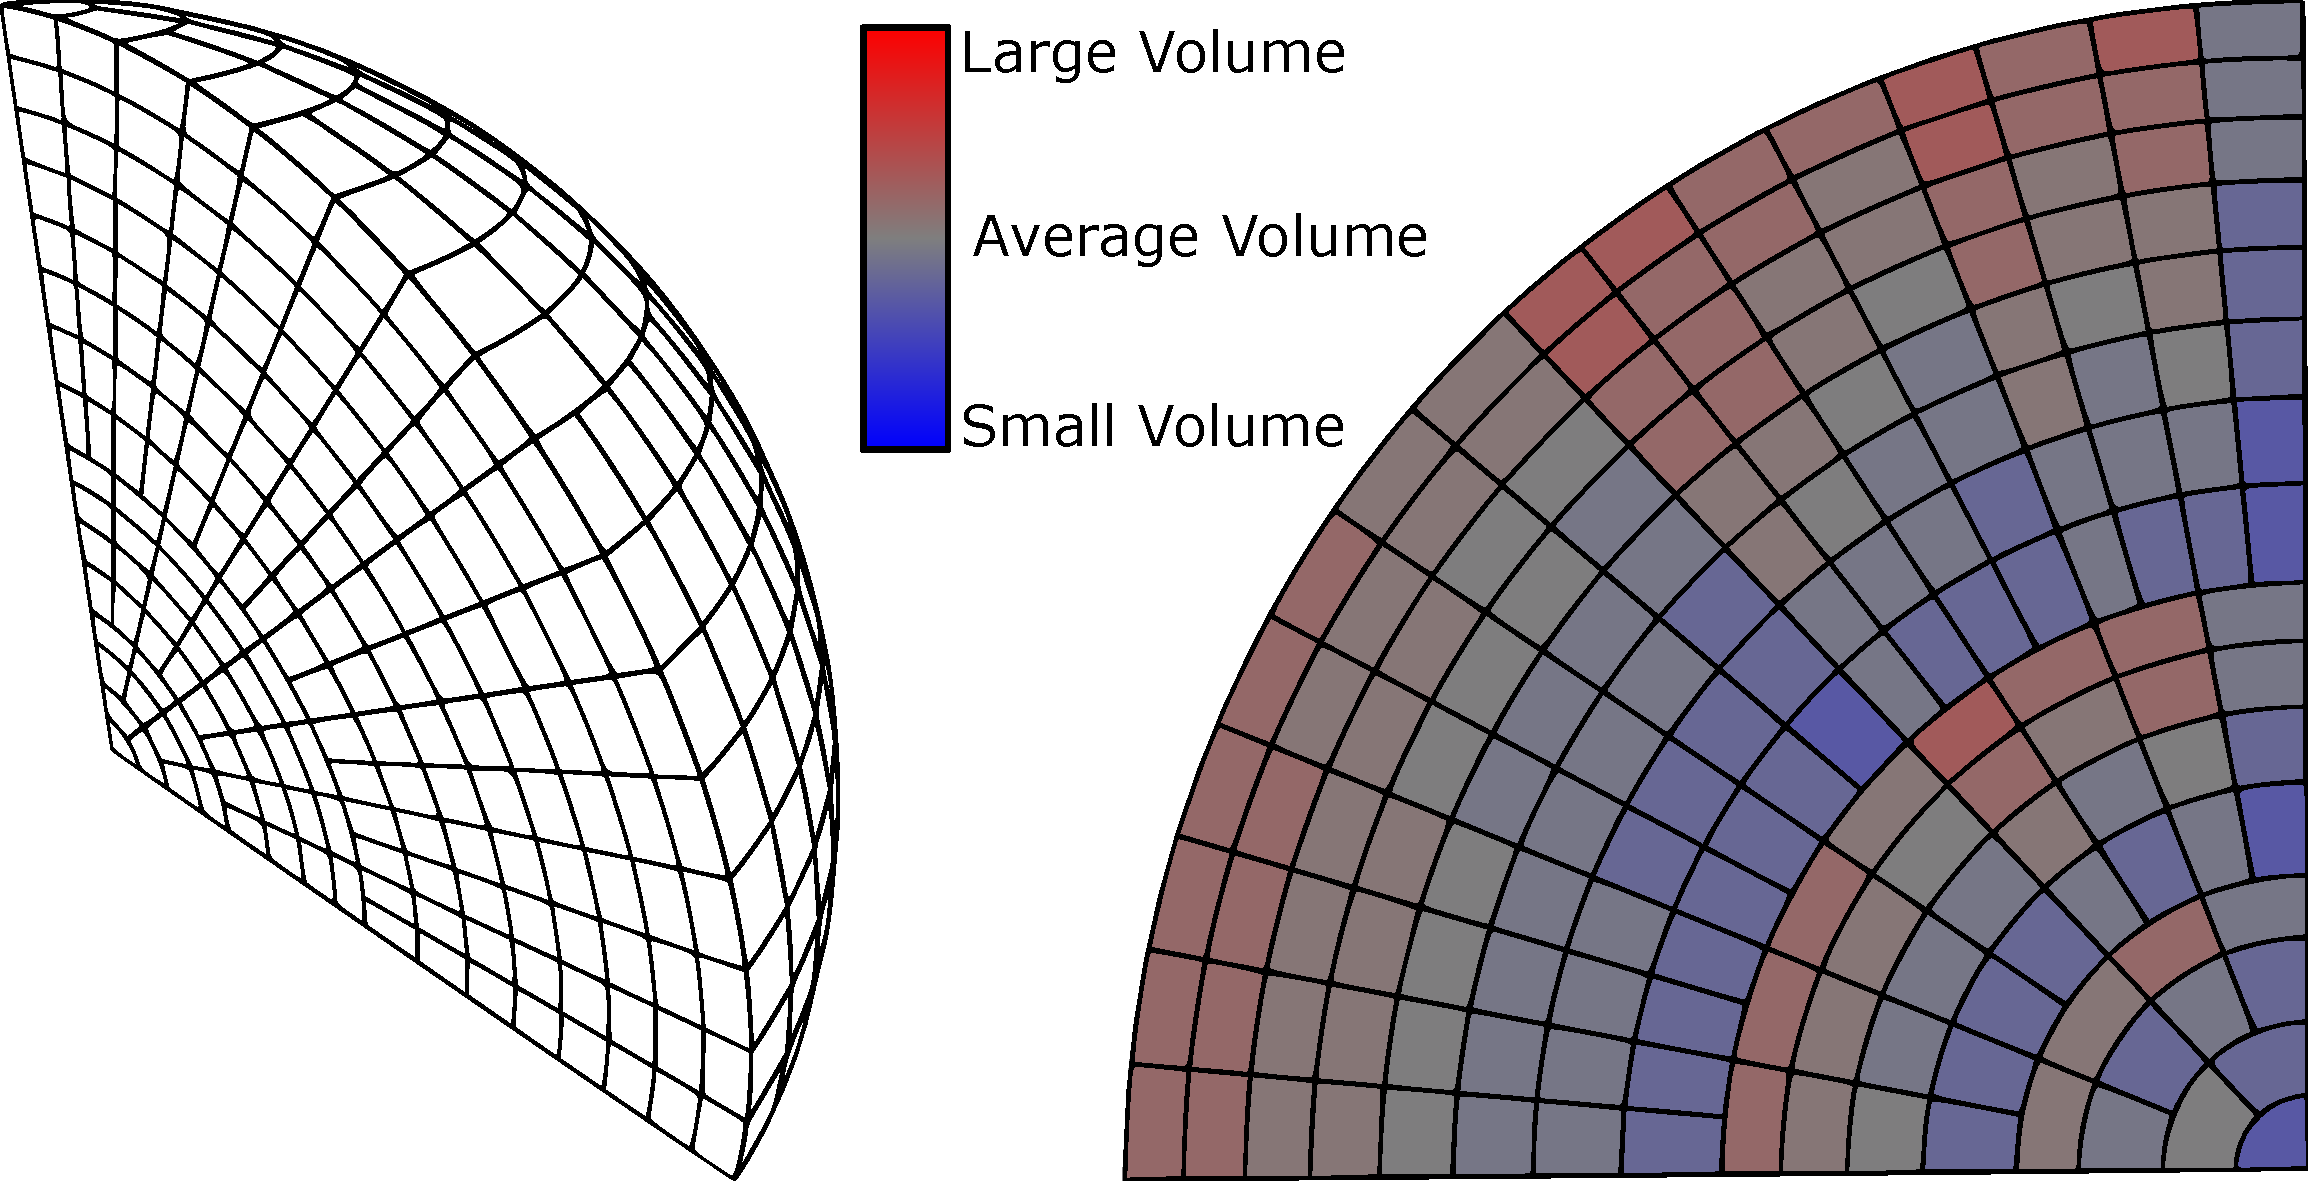
\includegraphics[width=0.85\textwidth]{Fig10.pdf}
	\caption{Results of the non-stationary scheme after four levels of subdivision using $\beta = \frac{1}{2}$.
		NG cells are still stretched and squashed in order to better preserve volume, however the effect is less pronounced}
	\label{fig:balanced}
\end{figure}


Figure~\ref{fig:perfect} shows the resulting grid from this method of calculating splitting surfaces.
In this grid, all NG cells at the same level of subdivision have exactly the same volume as one another.
This greatly improves the volume preservation, as only cells that extend to one of the poles (SG and LG cells) will have a different volume than the other cells in the grid.
This does not come without consequence though; cells are stretched and squashed in order to achieve this volume preservation, which may be an undesirable effect depending on the application.
To offset this reduction in cell compactness, it is possible to use splitting factors that are somewhere in between these ones ($c_{s}'$), which give ideal volume preservation, and the conventional SDOG ones ($c_{m}$), which give better compactness.
One simple way to calculate this would be as a convex combination of the two
%
\begin{equation}
c_{s} = \beta c_{s}' + \left( 1 - \beta \right)c_{m}, \quad \beta \in \left( 0,1 \right),
\label {eq:beta}
\end{equation}
%
however other methods could give better results.
We show a simple result in Figure~\ref{fig:balanced} using $\beta = \frac{1}{2}$.

\section{Results}
There are several potential methods for evaluating the volume preserving properties of a 3D DGGS.
When first proposed in \cite{yu2009sdog}, the ratio between cells of largest and smallest volume was used to evaluate volume preserving properties of SDOG.
This volume ratio is a useful measure for determining the worst-case difference in the volume of cells, however it does not give any information about the distribution of said volumes.
For example, a grid with all cells except one having equal volume, and a grid where every cell has a distinct volume, could end up having the same volume ratio.
To get a more complete understanding of volume preservation, we should also examine statistics that give a measure of distribution.
For this purpose, we use the coefficient of variation (CV), which is simply the ratio between the standard deviation and the mean.
We use the CV over the standard deviation as it a dimensionless quantity.


In modifying the subdivision for volume preservation, it is also important to evaluate the impact these changes have on other properties of the grid.
In Section \ref{sec:mapping} we discussed how the modified grids can be indexed using a mapping between them and conventional SDOG, however we should also measure the effect our changes have on the compactness of the resulting cells.
To measure this, we use the notion of sphericity, which quantifies how closely the shape of an object approximates a sphere~\cite{wadell1935volume}.
It is defined as the ratio between the surface area of a sphere with the same volume as the object and the surface area of the object itself.
Therefore, a perfect sphere will have a sphericity of one, and any other object will have sphericity strictly less than one.
Formally, given an object $\omega$ and a sphere $s$ such that $\operatorname{vol}(s) = \operatorname{vol}(\omega)$, the sphericity of $\omega$, $\Psi$, is given by $\frac{\operatorname{area}(s)}{\operatorname{area}(\omega)}$ , or equivalently 
%
\begin{equation}
\Psi = \frac{\pi^{\frac{1}{3}}\left( 6\operatorname{vol}(\omega) \right)^{\frac{2}{3}}}{\operatorname{area}(\omega)}.
\label{eq:sphericity}
\end{equation}
%
We use the mean and standard deviation (SD) of sphericity for all cells in the grid to evaluate compactness globally.


\begin{figure}[tbp]
	\centering
	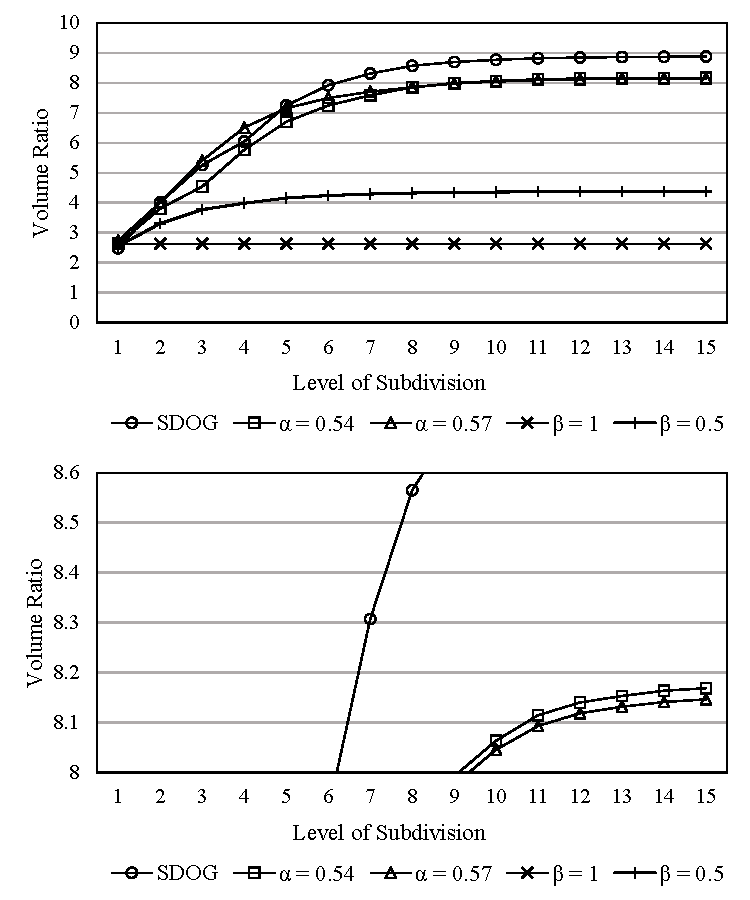
\includegraphics[width=0.75\textwidth]{Fig11.pdf}
	\caption{Volume ratio for the different grids at increasing levels of subdivision.
		Note that for the non-stationary method ($\beta = 1$) the volume ratio does not change with subdivision level}
	\label{fig:vr}
\end{figure}


\begin{figure}[tbp]
	\centering
	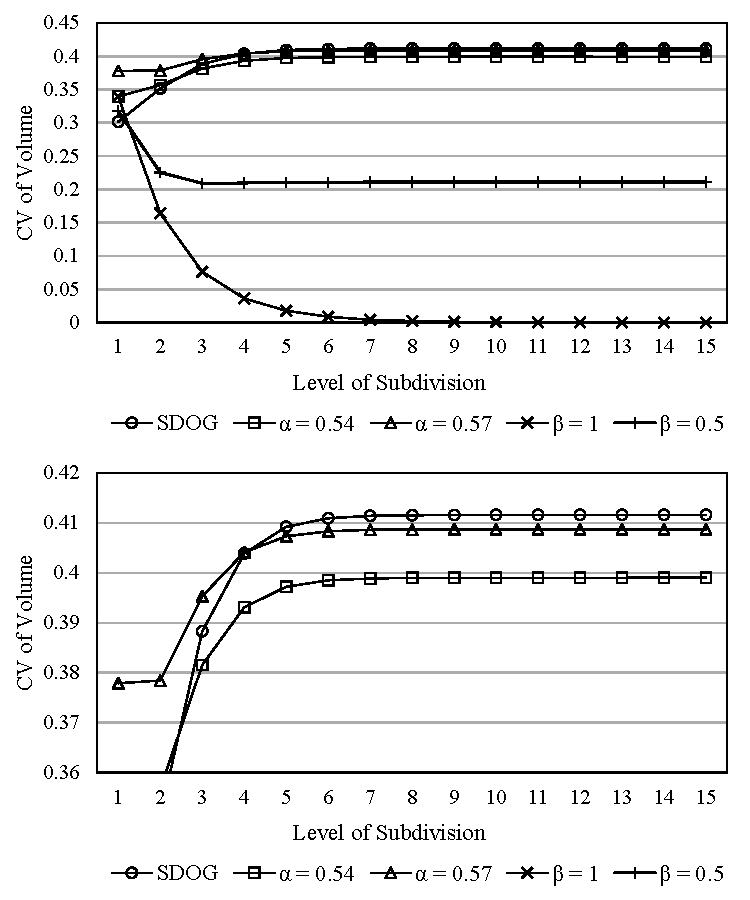
\includegraphics[width=0.75\textwidth]{Fig12.pdf}
	\caption{CV of volume for the different grids at increasing levels of subdivision}
	\label{fig:cv}
\end{figure}


\begin{figure}[tbp]
	\centering
	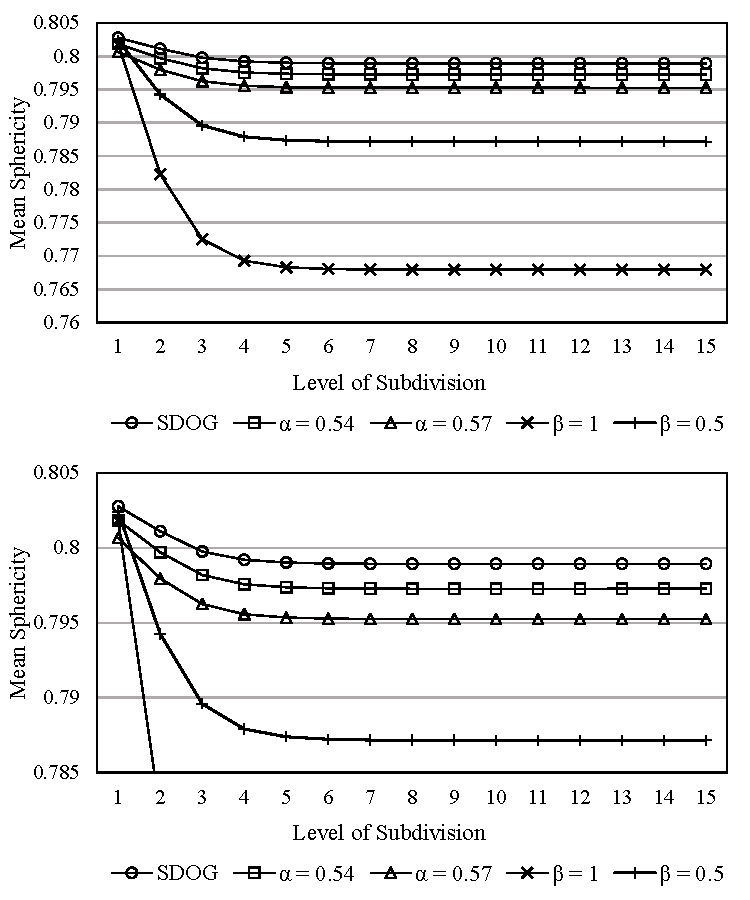
\includegraphics[width=0.75\textwidth]{Fig13.pdf}
	\caption{Mean sphericity for the different grids at increasing levels of subdivision}
	\label{fig:sph}
\end{figure}


\begin{figure}[tbp]
	\centering
	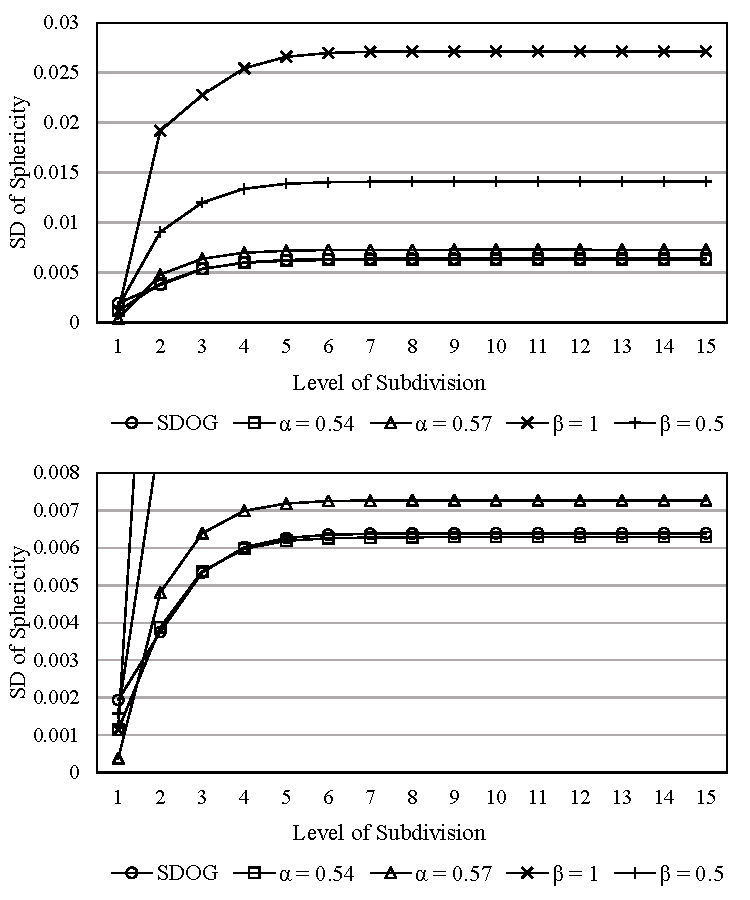
\includegraphics[width=0.75\textwidth]{Fig14.pdf}
	\caption{Standard deviation of sphericity for the different grids at increasing levels of subdivision}
	\label{fig:sd-sph}
\end{figure}


As a baseline, we have calculated the value of these measures at each subdivision level from one to fifteen for conventional SDOG.
We then repeated this for the four modifications discussed in this paper: the two stationary modifications with $\alpha_{\phi}^{SG} \approx 0.54$ and $\alpha_{\phi}^{SG} = 0.57$, the non-stationary modification (referred to as $\beta = 1$), and finally the blending of the non-stationary with conventional SDOG using $\beta = \frac{1}{2}$.
The results for each grid are displayed in Figures~\ref{fig:vr}, \ref{fig:cv}, \ref{fig:sph}, and \ref{fig:sd-sph} showing the volume ratio, CV of volume, mean sphericity, and SD of sphericity respectively.
Table~\ref{tab:results} summarizes these charts with the convergence value of each property for the five different grids.
We also give convergence values for the maximum and minimum sphericity---and their difference---for each grid in Table~\ref{tab:results-sph}.
It is important to note that for volume ratio and CV of volume lower values are better, but for mean sphericity a higher value is better.


\begin{table}[]
	\centering
	\caption{Convergence value of each measure for the five discussed grids}
	\begin{tabular}{|c|c|c|c|c|c|}
		\hline
		& SDOG & $\alpha_{\phi}^{SG} \approx 0.54$ & $\alpha_{\phi}^{SG} = 0.57$ & $\beta = 1$ & $\beta = 0.5$ \\ \hline
		Volume Ratio     & 8.88   & 8.17   & 8.15   & 2.63      & 4.37   \\ \hline
		CV of Volume     & 0.412  & 0.399  & 0.409  & 6.44E-19  & 0.211  \\ \hline
		Mean Sphericity  & 0.799  & 0.797  & 0.795  & 0.767     & 0.787  \\ \hline
		SD of Sphericity & 0.00639& 0.00629& 0.00727& 0.0271    & 0.0141 \\ \hline
	\end{tabular}
	\label{tab:results}
\end{table}


\begin{table}[]
	\centering
	\caption{Convergence value of max and min sphericity for the five discussed grids}
	\begin{tabular}{|c|c|c|c|c|c|}
		\hline
		& SDOG & $\alpha_{\phi}^{SG} \approx 0.54$ & $\alpha_{\phi}^{SG} = 0.57$ & $\beta = 1$ & $\beta = 0.5$ \\ \hline
		Max sphericity & 0.806  & 0.806  & 0.806  & 0.806 & 0.806  \\ \hline
		Min sphericity & 0.754  & 0.763  & 0.766  & 0.672 & 0.728  \\ \hline
		Difference     & 0.0520 & 0.0428 & 0.0404 & 0.134 & 0.0780 \\ \hline
	\end{tabular}
	\label{tab:results-sph}
\end{table}


The stationary scheme with $\alpha_{\phi}^{SG} \approx 0.54$ has a better volume ratio than conventional SDOG for all levels of subdivision except the first, and a lower CV of volume for all levels of subdivision after the second.
Comparing this to the one with $\alpha_{\phi}^{SG} = 0.57$, both the volume ratio and CV of volume do not improve as compared to conventional SDOG until the fifth level of subdivision.
Both of these methods also reduce the mean sphericity of cells at all levels of subdivision, with $\alpha_{\phi}^{SG} = 0.57$ having more than twice the absolute reduction of $\alpha_{\phi}^{SG} \approx 0.54$.
The variation in sphericity is similar between all three of these grids.
Using $\alpha_{\phi}^{SG} = 0.57$ does give a slightly better volume ratio than $\alpha_{\phi}^{SG} \approx 0.54$ as the level of subdivision gets large, however this difference is quite small and likely not worth the lower cell compactness and higher variation in volume.


The non-stationary scheme gives a much larger improvement to both the volume ratio and the CV of volume.
This is to be expected, as all NG cells in this scheme have exactly equal volume.
As the level of subdivision gets large, the CV of volume quickly approaches zero since the number of NG cells is much larger than the number of LG and SG cells in the grid.
The cost of this improved volume preservation is a much larger reduction in the sphericity of cells and an increase in the variation of sphericity, which is to be expected.
The blending scheme has results in between that of conventional SDOG and the non-stationary scheme, which was also expected.
The CV of volume, mean sphericity, and SD of sphericity are all near the respective halfway points, whereas the volume ratio still ends up being a significant improvement over conventional SDOG.

\section{Summary}